\documentclass{statsoc}
\usepackage{color, colortbl}
\usepackage[a4paper,showframe=false]{geometry}
\usepackage{graphicx}
\usepackage{psfrag,epsf}
\usepackage[textwidth=8em,textsize=small]{todonotes}
\usepackage{amsmath}
\usepackage{amsfonts}
\usepackage{natbib}
\usepackage{enumerate}
\usepackage{algorithm}
\usepackage{float}
\usepackage{color}
\usepackage{subfigure}
\usepackage[noend]{algpseudocode}
\algrenewcommand\algorithmicrequire{\textbf{Input:}}
\algrenewcommand\algorithmicensure{\textbf{Output:}}
\definecolor{Gray}{gray}{0.7}
\usepackage{hyperref}
\hypersetup{
    colorlinks=true,
    linkcolor=blue,
    filecolor=magenta,      
    urlcolor=blue,
}
\usepackage{changepage}
\usepackage{siunitx}

\title[Computing Confidence Intervals via Penalized Quantile Regression Splines]{Computing Confidence Intervals from Massive Functional Data via Penalized Quantile Regression Splines}
\author{Likun Zhang, Enrique del Castillo,}
\address{Pennsylvania State University,
State College,
USA.}
\email{lfz5044@psu.edu}
\author[L.Zhang, E.D.Castillo, A.J.Berglund, M.Tingley, and N.Govind]{Andrew J. Berglund, Martin Tingley and Nirmal Govind.}
\address{Netflix Inc.,
Los Gatos,
USA.}

\begin{document}


\begin{abstract}
The paper presents new methodology for the computation of pointwise confidence intervals from massive functional data sets. We utilize more robust and flexible quantile regression splines to allow heteroscedasticity and then estimate the functional form of any quantile level of the response. Our method introduces a new criterion for selecting the penalization coefficient, and incorporates, via bootstrapping and generating empirical confidence intervals, the variability of the fitted quantile function, including the uncertainty in the penalty coefficient. %Confidence bands on the fitted quantile functions can be used to compare the responses under different treatment and control experiences, and to estimate the treatment effect at different values of the covariates. 
To improve scalability of the method for massive datasets, the ``bag of little bootstraps" was adapted for quantile regression splines. Coverage analysis is presented to demonstrate 
the performance of the computed confidence bands or surfaces. An R package, {\tt ConfidenceQuant}, implements the new method. The approach has broad applications, including analysis of massive spatial data sets, analysis of large-scale computer model experiments, and analysis of experiments seeking to optimize the quality of video streaming over the Internet. We illustrate the methodology by comparing daily summertime maximum temperature projections from NASA's Earth Exchange climate models. We consider two different CO${_2}$ emissions scenarios, and compare projections over the continental United States for the mid and late 21st Century, respectively. 
%In total, each comparison involves 12.6 million data points.

\textit{Keywords:}  Quantile regression, penalized splines, confidence intervals, bag of little bootstraps, massive functional data.
\end{abstract}


\section{Introduction}\label{s1}
Quantile regression methods provide a more robust approach for examining functional changes than models based on conditional means \citep{koenker2005quantile}, with the functional forms running the gamut from linear to penalized methods that result in flexible smoothing splines. More often than not, inferences on properties of the conditional distribution other than the mean, such as a median or an extreme quantile, are of great interest because different quantiles offer a more complete view of the response variable. Since assumptions of normality do not always apply, a nonparametric approach like bootstrapping may be required to incorporate the sample variability of the fitted quantiles. For larger data sets, traditional bootstrapping is not always sufficient due to the poor scalability and the prohibitive computational cost.

Here we propose to adapt the ``bag of little bootstraps" (BLB) method by \citet{kleiner2014scalable} to provide uncertainty estimation for penalized quantile regression spline models applied to very large data sets. Although flexible Bayesian approaches for quantile regression models have been proposed in recent years \citep{Reich2010,Yang2012}, the required MCMC computations are not amenable to the analysis of the massive data sets we intend to study. The main advantage of BLB is that it takes on a modern parallel and distributed architecture while preserving the statistical efficiency of the bootstrap. Another methodological objective of this paper is to propose a new algorithm to automate the selection of the smoothing parameter in penalized quantile regression splines. The existing criteria for choosing the tuning parameter that controls the smoothness of the functional estimate generally relies on the calculation of the effective degrees of freedom of quantile fit, which we found to be intractable and problematic for data sets of any size; see section \ref{refintro} for details. Our proposed criterion, based on a cross-validation technique, is well-behaved and selects a smoothing parameter that achieves a desirable balance between the smoothness of the fitted function and fidelity to the observed data points.

This paper was motivated by large-scale ``A/B", or treatment-control experiments at Netflix aimed at improving the streaming video experience. Streaming experimentation at Netflix focuses on understanding and improving video ``quality of experience" -- ideally, playback will commence quickly (low play delay), feature high image quality, and have a low rate of rebuffer interruptions. For a general overview of work in this area, see \citet{govind2014optimizing, govind2017A/B}. Many of the streaming video experiments conducted at Netflix feature treatment effects that are heterogeneous with respect to network conditions. For example, proposed changes to the adaptive streaming algorithm may attempt to reduce play delay for low bandwidth networks, or aim to reduce rebuffer interruptions by making more conservative bitrate selections for highly variable network connections. In this context, we are interested in flexible conditional quantile models: for example, has an experimental treatment reduced the upper quantiles of play delay, and does that reduction vary with measures of network bandwidth and variability? 

The methodology developed in this paper has wide applicability, and as Netflix data is proprietary, we turn to open source data from climate modeling experiments as an example application. In particular, we consider predictions of surface temperatures in the continental United States at the end of 21st Century under representative concentration pathways (RCP) 4.5 and 8.5 \citep{van2011representative}, respectively. These data sets feature the required scale, with each RCP yielding more than 12.6 million   {data points}, while the spatial nature permits for a demonstration of our methodology with two covariates. 

The remainder of this paper is organized as follows. Section \ref{s2} introduces the nonparametric quantile smoothing spline model. Model fitting is via a penalized objective that controls the smoothness of the fitted  quantile function, and the selection of the penalization parameter is based on the Multifold Cross-Validation approach by \citet{reiss2012smoothness}. Section \ref{s3} describes the computation of pointwise confidence bands (or surfaces) around the nonparametric quantile regression function using the ``bag of little bootstraps" method \citep{kleiner2014scalable}, and section \ref{lambdasel} discusses a new criterion and the selection of the smoothing (penalization) parameter given the distributed nature of the ``bag of little bootstraps" method. A coverage analysis of the performance of the method on various simulated functions and surfaces is presented in section \ref{s5}. Finally, the methodology is used to compare open source climate model predictions in section \ref{s6}.
%observations.[not ideal as they are simulated.]

\section{Nonparametric quantile regression}\label{s2}
\subsection{Quantile smoothing splines}\label{s21}

Our interest in using nonparametric quantile smoothing splines stems from the more flexible functional forms they provide compared to the parametric models, as well as their robustness to outliers and very few assumptions about the distribution of errors. For a thorough discussion of nonparametric quantile regression, see \citet{koenker2005quantile,koenker1978regression}. In the case where there is only one covariate, given a sample of $n$ individuals with predictors $x_1,\cdots, x_n$, responses $y_1,\cdots, y_n$, and a quantile $\tau \in [0,1]$ of interest, the penalized quantile regression entails solving the penalized minimization problem:
\begin{equation}
\label{prob}
    \min_{g\in \mathcal{G}}\sum_{i=1}^n \rho_{\tau}[y_i - g(x_i)] + \lambda J(g),
\end{equation}
where $\rho_{\tau} (u) = u\{\tau-I(u<0)\}$ is the ``check function", $J(g)$ is a given roughness functional, and $\lambda>0$ is a tuning factor that determines the smoothness of the fitted function $g$. The solution yields the conditional $\tau$th quantile of $y$ as a function of $x$, with the penalized objective trading off the {\it fidelity} of the fitted function (first term) with some measure of its {\it roughness} (second term). Different types of penalty functions, such as $L_p$ penalties, have been studied in the literature \citep{cox1983asymptotics,bosch1995convergent}. \citet{koenker1994quantile} reformulated the $L_1$ roughness penalty term, $\int |g''(x)| dx,$ in terms of the total variation of the function $g'$, which is defined by maximizing over all partitions $a\leq s_1<\cdots<s_n<b$ of the interval $[a,b]:$
\begin{equation}
\label{totalvar}
    V(g') = \sup \sum_{i=1}^n |g'(s_{i+1})-g'(s_i)|,
\end{equation}
where $g\in \mathcal{G}$ is a function with absolutely continuous first derivative. The function $V(g')$ is well-defined for a larger set of functions than the $L_1$ penalty. The solution $\hat{g}$ to problem \eqref{prob} under the total variation penalty \eqref{totalvar} is proved in \citet{koenker1994quantile} to be a piecewise linear function with knots at  {each} observed $x_i$,  {$i=1,\cdots,n$}. Problem \eqref{prob} can thus be reformulated as a finite-dimensional linear programming (LP) problem \citep{koenker1994quantile},   {allowing these models to be fit to large datasets}. 

For $g : \mathbb{R}^2 \rightarrow \mathbb{R}$ (two dimensional covariates), \citet{koenker2004penalized} generalized the total variation roughness penalty $J(g)=V(g')$ to the bivariate setting by calculating the variational integral $V(\nabla g) = \int ||\nabla^2g(x)||dx$, where $||\cdot||$ denotes the Frobenius norm \citep{serrin1961definition}. Restricting the domain of functions $\mathcal{G}$ to piecewise linear functions over a specified triangulation (i.e., triograms,  {see section \ref{weights} below}), problem \eqref{prob} can be again reformulated as a linear programming problem. A modified version of the Frisch-Newton algorithm, which implements the log barrier interior point method, can then solve the problem efficiently \citep{koenker2005frisch}.

Extending the penalized quantile regression model to more than two covariates is hard due to the fundamental difficulty to generalize the total variation roughness penalty $V(\nabla g)$ for multivariate functions; it is also challenging to build multivariate spline bases that lead to orthogonally equivariant fitted functions (see \citet[p. 235]{koenker2005quantile}). In this paper, we only focus on univariate and bivariate quantile smoothing. \textcolor{blue}{[Maybe explain more why our method, which can only model covariates up to two dimensions, can be useful by further discussing experimentation applications at Netflix?]}

\subsection{Previous approaches to selecting the smoothing parameter}\label{refintro}

Fitting a penalized quantile smoothing spline \eqref{prob} requires that the value of the smoothing parameter $\lambda$ be specified. Various methods have been proposed in the literature to automatically select an ``optimal" value of $\lambda$ for nonparametric regression \citep{akaike1973problems,schwarz1978estimating}. \citet{koenker1994quantile} suggested what is perhaps the most popular method, a variant of Schwartz's Information Criterion (SIC):
\begin{equation}
    \mbox{SIC}(\lambda)=\log\left(\frac{1}{n} \sum_{i=1}^n \rho_{\tau}\{y_i - \hat g_{\lambda}(x_i)\}\right) + \frac{\log n}{2n}p(\lambda),
\end{equation}
 where $p(\lambda)$ is the effective degrees of freedom of the fit, defined as the number of `active' knots that are interpolated by the fitted function (i.e., the number of zero-valued residuals). For univariate smoothing, Koenker et al. suggested that  $p(\lambda)-1$ is equivalent to the number of distinct linear segments of the fit, and that therefore it should provide a useful index of the smoothness of the fitted curve. The concept of SIC is intuitive: as $\lambda$ decreases to zero, the fidelity term dominates the objective function in \eqref{prob} more. To solve \eqref{prob}, $\hat g_{\lambda}(x_i)$, the fitted function at each point $x_i$, will become closer to the data $y_i$, which means more distinct linear segments. This will make the log term in SIC smaller and $p(\lambda)$ larger. In the end, the $\lambda$ value that minimizes the SIC function can be considered to be an optimal smoothing parameter.
 
 We have found $p(\lambda)$ to be an intractable measure of smoothness, however, because in fact $p(\lambda)-1$ is not equivalent to the number of distinct linear segments, especially for large datasets. To determine $p(\lambda)$, we must count how many residuals $u_i=y_i-\hat g_{\lambda}(x_i)$ are less than a numerical tolerance in absolute value;  the probability that there are more numerically zero residuals increases with the number of data points, and will vary erratically with small variations in $\lambda$ as the linear segments may have minute changes in slopes and intercepts, making $p(\lambda)$ an inadequate measure of roughness.  To illustrate, Figure \ref{fig:edf} shows 5,000 simulated samples from a simple parabolic model to which we fit a median function using quantile smoothing splines with two different but very close $\lambda$ values  {(0.008 and 0.0085)}. The two quantile functions fitted with these $\lambda$ values have  $p(\lambda)$  values equal to 160 and 43, respectively, which by definition give the number of interpolated points for each model fit.  By contrast, the number of linear segments in each case is 158 and 167, while the sum of the fidelity terms are 956.58 and 957.31, indicating very similar fits. This demonstrates how small changes in $\lambda$ can result in large changes in the number of zero residuals accounted by $p(\lambda)$, with almost no effect in the smoothness of the fitted quantile.  
\begin{figure}
\centering   
  \subfigure[$\lambda=0.008,p(\lambda)=160$]{\label{fig:a_new}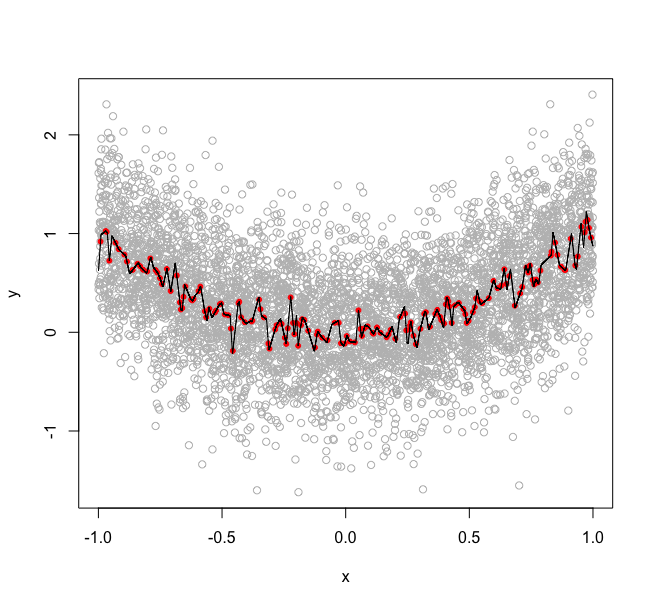
\includegraphics[width=70mm]{1-21.png}}
  \subfigure[$\lambda=0.0085,p(\lambda)=43$]{\label{fig:b_new}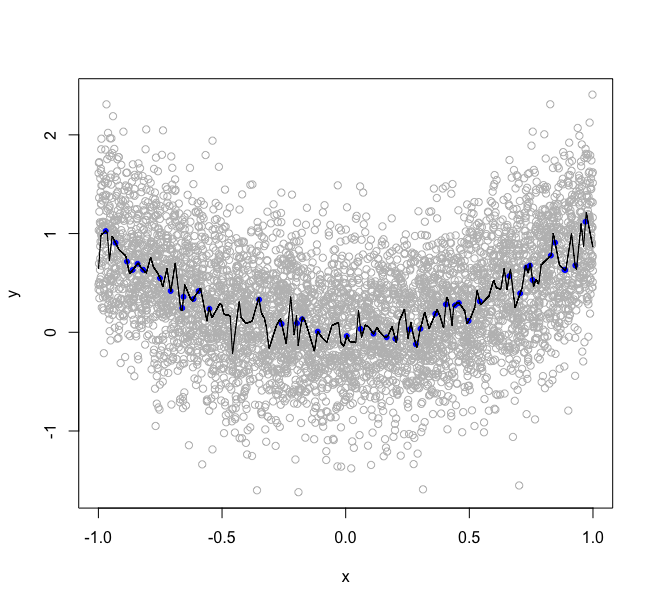
\includegraphics[width=70mm]{2-23.png}}
\caption{Simulated data set with 5,000 samples. True underlying model is $y_i=x_i^2+\epsilon_i,\text{ where }\epsilon_i\stackrel{iid}{\sim} N(0,0.5^2)$, and $x_i$ covariates are sampled uniformly from [-1,1]. The  {solid lines} show fitted quantile smoothing splines for $\tau=0.5 \text{ (median)}$ using slightly different (and non-optimal) $\lambda$ values. The red and blue  {dots are points} interpolated by the two fitted median functions (i.e., points with zero residuals). Despite the similarity of the two function estimates, the corresponding numbers of interpolated points differ greatly, indicating $p(\lambda)$ varies considerably for fitted curves that have,  {to the eye} a very similar degree of smoothness. Compare with Figure \ref{fig:fitted}.}
\label{fig:edf}
\end{figure}

Figure \ref{fig:SIC} includes the $p(\lambda)$ and SIC values calculated for a grid of $\lambda$ values on $[0,0.1]$ for the same data set as in Figure \ref{fig:edf}. We can see that neither $p(\lambda)$ nor the SIC functions are  smooth. As $\lambda$ increases to sufficiently large values, the roughness penalty dominates the fidelity objective in \eqref{prob} until one obtains the limiting simple linear fit with $p(\lambda) = 2$ and a single linear segment. With a linear function being the solution for large $\lambda$, the fidelity term will not increase and accordingly the SIC will flatten out for increasingly larger $\lambda$. Both the erratic behavior in $p(\lambda)$ and the non-convexity of SIC($\lambda$) make it difficult to optimize SIC no matter how fine the grid of $\lambda$ values are. Hence SIC, based on $p(\lambda)$,  a count of residuals smaller than a threshold, is not a useful criterion for selecting the best $\lambda$ smoothing constant.

\begin{figure}[H]
\centering   
  \subfigure{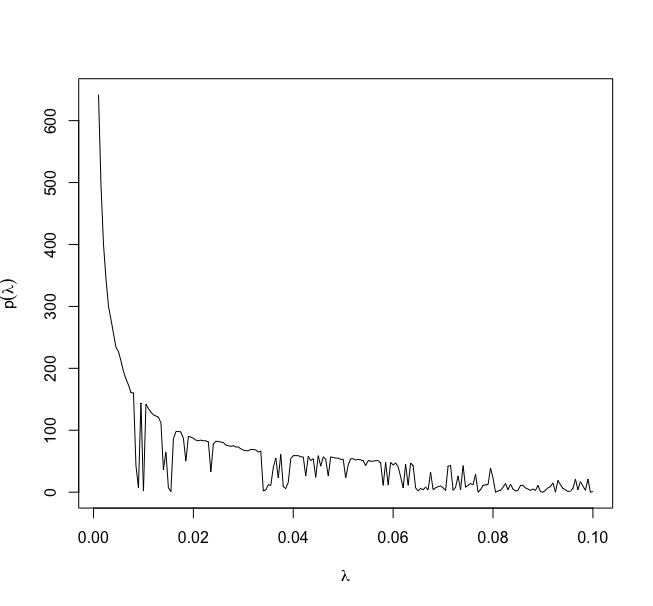
\includegraphics[width=70mm]{edf.png}}
  \subfigure{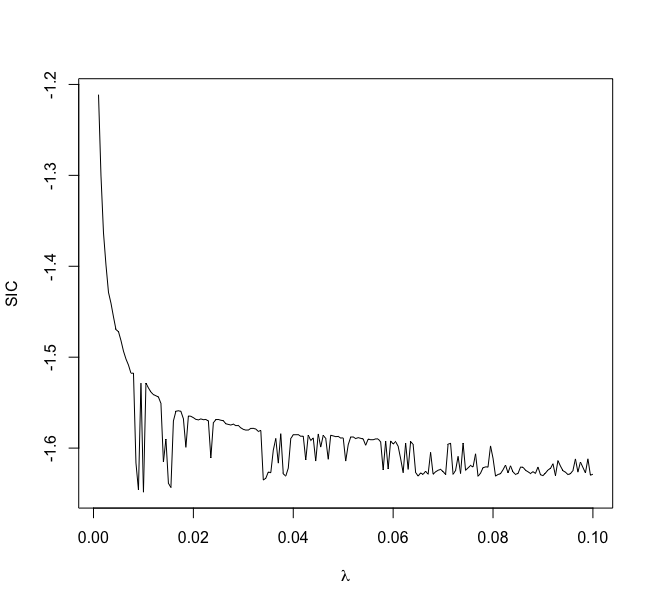
\includegraphics[width=70mm]{sic.png}}
  \caption{The $p(\lambda)$ (left) and SIC$(\lambda)$ function (right), calculated for the same data set as shown in Figure \ref{fig:edf} ($\tau=0.5$).}
\label{fig:SIC}
\end{figure}

Cross-validation, another commonly used technique for selecting the smoothing parameter in quantile spline models, was investigated by \citet{yuan2006gacv}. The simple idea is to use leave-one-out function estimates to calculate a cross-validation score, which is referred to in the literature as robust cross-validation (RCV) \citep{oh2004period}:
  \begin{equation}
     \label{RCV}
     \text{RCV}(\lambda)=\frac{1}{n} \sum_{i=1}^n \rho_{\tau}[y_i-\hat{g}_{\lambda}^{[-i]}(x_i)],
 \end{equation}
where $\hat{g}_{\lambda}^{[-i]}(x_i)$ is the fitted function obtained without the $i$th observation. Objective \eqref{RCV} is computationally formidable since we have to evaluate $n$ quantile splines for each candidate smoothing parameter $\lambda$. \citet{nychka1995nonparametric} proposed an approximate cross validation (ACV) criterion as an approximation to RCV. The main idea is to pick a $\lambda$ value such that the distance between the resulting estimate and the true function is minimized. To further reduce the computational expense, \citet{yuan2006gacv} proposed a generalized approximate cross-validation (GACV) criterion to improve upon ACV.  Unfortunately, the approximate forms of both ACV and GACV, which are easier to calculate, rely on $p(\lambda)$, and hence are too erratic to be optimized as a function of $\lambda$. 
 
To alleviate issues associated with the erraticism of $p(\lambda)$, we adopted a Multifold Cross-Validation (MCV) approach for the selection of $\lambda$. Our approach is similar to that of Reiss and Huang \citep{reiss2012smoothness}, who proposed an MCV statistic for finding the optimal smoothing parameter in quantile smoothing splines under a {\it quadratic} penalty function. For such penalty, they show evidence that MCV provides better performance than other methods, including SIC. We apply MCV for finding $\lambda^*$ in quantile spline smoothing using instead the total variation penalty function as described in section \ref{s21}.
  
The Reiss and Huang MCV statistic is defined by:
\begin{equation}
    \mbox{MCV}(\lambda)=\frac{1}{n}\sum_{j=1}^{K} \sum_{i\in V_j} \rho_{\tau}[y_i-\hat{g}_{\lambda}^{[-V_j]}(x_i)],
    \label{MCV}
\end{equation}
where $V_1, \ldots, V_{K}$ are the $K$ equal-sized parts (folds) of the original data, and $\hat{g}_{\lambda}^{[-V_j]}$ denotes the smoothing spline fitted to all folds except fold $V_j$ (the training set). The recommended number of folds in cross validation ranges from 5 to 10 \citep{reiss2012smoothness}.  

The graph on the left of Figure \ref{fig:fitted} displays the MCV function (10 folds) plotted over $\lambda$ values in $[0,4.0]$ for the same data set as used in Figure \ref{fig:edf}. The MCV$(\lambda$) function is  {better behaved than the SIC function, offering an easier criterion to locate the minimum and find an optimum smoothing parameter $\lambda^*$, recovering the desired property similar to the quadratic}. The corresponding fitted median shown on the right of Figure \ref{fig:fitted} approximates the true median function very well, according with our intuition. In contrast, the $\lambda$ parameters used in Figure \ref{fig:edf} are much smaller, resulting in under-smoothed quantile functions. The excellent behavior of the MCV$(\lambda)$ method was corroborated over many other simulated data sets, and we therefore adopt and modify this criterion in section \ref{lambdasel} to make it suitable to the distributed nature of the ``bag of little bootstrap" method. 
\begin{figure}
\centering   
  \subfigure[$\lambda^*=0.541,\text{MCV}(\lambda^*)=0.19765$]{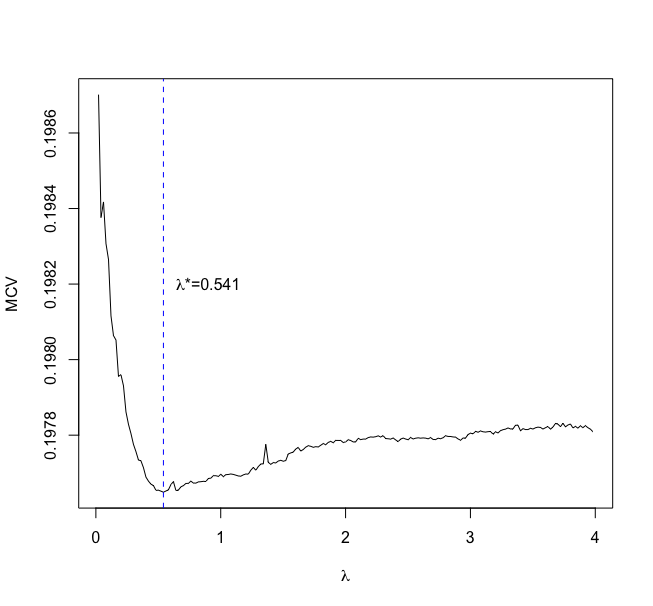
\includegraphics[width=70mm]{MCV_3000.png}}
  \subfigure[Fitted median function]{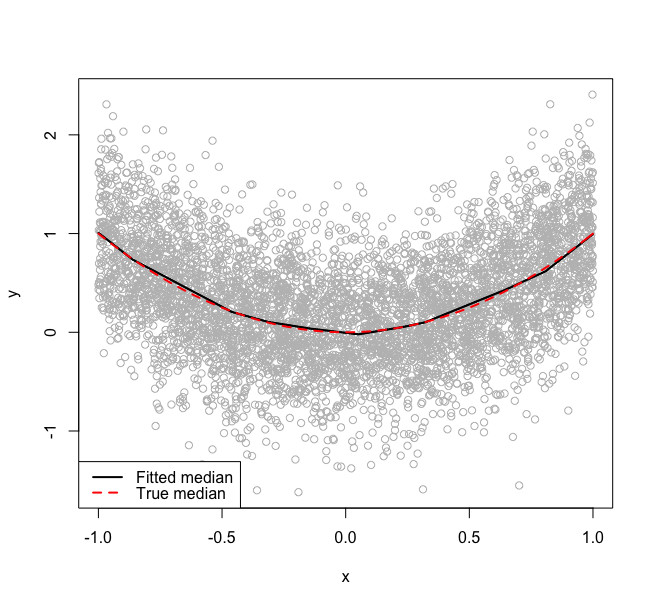
\includegraphics[width=70mm]{fitted.png}}
\caption{ {(a): MCV$(\lambda)$ function ($\tau=0.5$) for the same data set as shown in figure \ref{fig:edf}. (b): The optimum smoothing parameter $\lambda^*$ results in the displayed fitted median function.}}
    \label{fig:fitted}
\end{figure}

\section{Bootstrap confidence bands for nonparametric quantile regression}\label{s3}
\subsection{Bootstrapping and the ``big data" problem}

After estimating a quantile curve in a flexible nonparametric way, we wish to understand whether an observed peak or valley reflects the underlying true quantile function or if it is only an artificial effect introduced by the experimental errors. Examining the confidence intervals of the curves (or surfaces) at a grid of points can offer a direct assessment of where in the space of the covariates the observed features are significant. The use of bootstrap methods is common for determining confidence bands in nonparametric regression without recourse to any distributional assumptions \citep{mcdonald1982interactive,dikta1990bootstrap}. \citet{hardle1991bootstrap} proposed a method that gives the confidence bands for the fitted mean curves by resampling from estimated residuals. However, the residual bootstrap is  {not appropriate in our context} because we need to assume i.i.d. errors and a location-shift model (see the explanation in \citet[p. 105]{koenker2005quantile}). This is unrealistic in many applications, especially when the residuals are heteroskedastic. In comparison, the na\"{i}ve approach of drawing from the sample pairs $\{(\mathbf{x}_i,y_i):i=1,\cdots,n\}$ with replacement works under independent but not identically distributed settings, offering an effective approach to approximating the variability of the quantile estimates \citep{dikta1990bootstrap}.

For small data sets ($n\sim 5k$), our experiments show that the bootstrap provides well-behaved confidence bands that have coverage probabilities similar to the desired confidence level. However, the very large size of the datasets we wish to analyze in the large-scale experiments at Netflix poses immediate difficulties if bootstrapping methods are to be applied. When sampled with replacement, each resample has size on the same order as the original data set, with nearly $(1-e^{-1})\%\approx 63\%$ of all the values appearing at least once in each resample. Since the execution time of solving problem \eqref{prob} using linear programming techniques grows exponentially with the number of unique values at the rate of around 1.54 (see \citet{koenker2005frisch}), computation of even one point estimate of the quantile function would be rather time-consuming for large $n$. Therefore repeated estimations for each resample would be prohibitively costly.

To improve the efficiency of the bootstrap, \citet{bickel2008choice} discussed the so-called $m$ out of $n$ bootstrap in which each bootstrap sample is only of size $m<n$. Although this method eases the computational complexity, the outputs are sensitive to the choice of the resample size $m$. Additionally, the estimators are repeatedly computed on resamples that are much smaller than the original data set, and thus they need to be rescaled so that the variability on the full data set is taken into account. 

We therefore adapt the ``Bag of Little Bootstraps" (BLB) method introduced by \citet{kleiner2014scalable}, a robust, efficient, and parallelizable procedure that combines subsampling and bootstrapping, to compute confidence bands (or surfaces) for quantile smoothing splines. Unlike the $m$ out of $n$ bootstrap, the BLB method resamples from small non-overlapping subsamples to form bootstrapped samples each of size $n$, matching the original data set. In this way, we are fitting quantile smoothing splines on full-sized data sets while in effect the computational cost is determined by the size of the small subsamples, given that quantile smoothing splines can work directly with the weighted (binned) representation of the bootstrapped samples. In the next sections we describe in detail how BLB was implemented for quantile smoothing regression, including a description of a new cross-validation method for selecting the smoothing constant $\lambda$ that exploits the computational advantages afforded by the BLB subsamples. 

\subsection{Distributed bootstrapping for massive data}
\subsubsection{Bag of Little Bootstraps (BLB) and quantile regression}

The BLB method method applied to quantile smoothing splines can be summarized in three steps. 1) Sample $s$ disjoint subsets or ``bags" each of size $b$ from the original $n$ data set uniformly. Values $b=n^{\gamma}$ with $\gamma\in (0.5,0.9)$ are recommended for the size of each bag, see \citet{kleiner2014scalable}. 2) From each bag, form $r$ bootstrap samples each of size $n$ points. Fit the quantile smoothing splines to each bootstrap sample for a given quantile $\tau\in (0,1)$ of interest. Then calculate pointwise bootstrap percentile intervals to obtain confidence bands for the quantile function. 3) Average the $s$ confidence bands obtained from bootstrapping each bag (see Algorithm \ref{BLB} for more details).

A major advantage of BLB is that we can parallelize the bootstrapping for $s$ bags and therefore a distributed computing architecture can be used for markedly larger datasets. Since $b<n$, the bootstrap samples obtained via resampling each bag will have repeated data points, and therefore they can be represented by a histogram with the unique observed numbers and the counts (frequencies or ``weights"), rather than using the raw data containing all repeated data. By reformulating the quantile estimation problem to work with the the weighted representation of the data, we can exploit the BLB speed gains and storage space savings.

Considering that we will repeatedly fit quantile smoothing spline models as part of BLB, it is helpful to quantify the computational complexity of a single model fit. To exploit the sparse structure of large problems, \citet{koenker2005frisch} applied sparse Cholesky factorization to the Frisch-Newton algorithm for quantile regression, which substantially reduces storage requirements and increases computation speed compared to a standard dense algorithm. As a result, they found out that the log execution time to obtain the penalized triogram solution is linearly dependent on the log of sample size. Therefore when we decrease the bootstrap sample size from $n$ to $b$ due to the application of the BLB method, the execution time will drop exponentially.  

\begin{algorithm}
\caption{Bag of Little Bootstraps (BLB\citep{kleiner2014scalable}) for quantile regression confidence bands}\label{BLB}
\begin{algorithmic}[1]
\Require \begin{tabular}{ll}
     Data $\mathbb{X}=\{(\mathbf{x}_i,y_i);i=1,\cdots,n\}$\qquad\qquad&$b$: size of subsets or `bags'\\
    $\tau$: quantile of interest&$s$: number of subsets or `bags'\\
   $\alpha$: significance level&$r$: number of bootstraps of each subset\\
   &$\lambda$: specified smoothing parameter
\end{tabular}
\Ensure Estimated confidence intervals for the $\tau$th quantile function
   \State Shuffle $\{1,\cdots,n\}$ and partition the set into disjoint subsets of size $b$ 
   \State Choose the first $s$ subsets: $\mathcal{I}_1,\cdots,\mathcal{I}_s$\Comment{Each subset has $b$ indices}
   \For {$j \leftarrow 1, s$}
      \State Generate a subset or `bag' $\mathbb{B}$ by subsetting $\mathbb{X}$ using indices $\mathcal{I}_j$
      \For {$k \leftarrow 1, r$}
         \State Sample $(w_1,\cdots,w_b)\sim \text{Multinomial}(n,\mathbf{1}_b/b)$ \Comment{Counts or weights}
         \State Obtain the bootstrap sample: $\mathbb{H}=\{\mathbb{B}\text{ weighted by }(w_1,\cdots,w_b)\}$\label{blah2}
         \State Fit quantile smoothing splines on $\mathbb{H}$ with $\lambda$ and get the $\tau$th quantile function\label{blah}
      \EndFor
      \State Calculate $(1-\alpha)$\% empirical confidence bands $(L_j,U_j)$ for the quantile function
   \EndFor
   \State $(L,U) \leftarrow \frac{1}{s}\sum_{j=1}^s{(L_j,U_j)}$ \Comment{Average the $s$ confidence bands}
\end{algorithmic}
\end{algorithm}

Another desirable feature of BLB is that it retains the statistical efficiency of the simple bootstrap. \citet{hall2013bootstrap} showed how the bootstrap estimates of quantiles are higher-order correct in many cases, which means that the bootstrap output converges to the true values at a rate of $O_P(1/n)$ or faster. To ensure the same degree of higher-order correctness for BLB, $s$ and $b$ need to satisfy $s\sim (n/b)$ and $b=\Omega(\sqrt{n})$ (see Theorems 2 and 3 in \citet{kleiner2014scalable}). Although $b$ may be significantly smaller than $n$, $b\times s$ should be on the same scale as $n$, meaning that all information from the original data set should be included in the analysis in order to maintain a fast convergence rate. Even though \citet{kleiner2014scalable} suggested that fairly modest values of $b$ and $s$ will suffice for BLB to reach relatively high accuracy, in what follows we ensure that $b\times s\approx n$ so that the asymptotic property is maintained.

\subsubsection{Implementing quantile smoothing splines using a binned (or weighted) data representation}\label{weights}
 
\citet{koenker2007quantreg} implemented their algorithm for fitting quantile smoothing splines in the R function {\tt rqss} of the {\tt quantreg} R package, a function for additive quantile regression models with possible univariate and/or bivariate nonparametric terms estimated by total variation regularization. Unfortunately, binned or histogram representations of data cannot be passed to the {\tt rqss} function, as its {\tt weights} argument is not   {operational}\footnote{Private communication with Professor Koenker.}.
As described next, we were able to `activate' the {\tt weights} functionality after studying the Frisch-Newton algorithm \citep{koenker2005frisch}, and hence we were able to speed up the bootstrap computations. 

For bivariate smoothing, \citet{hansen1998triogram} introduced continuous, piesewise linear functions defined over adaptively selected triangulations in the plane as a general approach to bivariate density estimation, generalized linear models, and proportional hazards regression. These functions, also called triograms, are analogous to linear interpolations at the knots in a univariate spline space. As briefly mentioned in section \ref{s21}, the domain of possible solutions to problem \eqref{prob} in the bivariate case, $\mathcal{G}$, is restricted to a class of piecewise linear functions over a specified triangulation, whose total variation proves more tractable (see \citet{koenker2004penalized}). Problem \eqref{prob} can thus be reformulated as:
\begin{equation}
    \label{tri}
    \min_{\boldsymbol{b}\in \mathbb{R}^n}\sum_{i=1}^n \rho_{\tau}[y_i - \boldsymbol{g}_i^T\boldsymbol{b}] + \lambda\sum_{k=1}^{M} |\boldsymbol{a}_k^T\boldsymbol{b}|
\end{equation}
while fixing the triangulation in the space of the two covariates (in the case of one covariate, such triangulation corresponds to the intervals between the $x_i$ values). In this reformulation, $\boldsymbol{g}_i$ denotes a  design vector with elements $g_{ij}=B_j(\boldsymbol{x}_i)$, with $\boldsymbol{x}_i$ being the covariates for the $i$th observation, and $B_j$ equal to the barycentric basis functions \citep{koenker2004penalized}, $j=1,\cdots,p$, where $p$ is the number of vertices in the triangulation. The elements in $\boldsymbol{b}$ represent the values that the fitted function $g$ takes at the vertices of the triangulation. The vectors $\boldsymbol{a}_k$ reflect the contribution of the $k$th interior edge to the total roughness of the function $g$, and $M$ is the total number of interior edges in the triangulation. To reformulate problem \eqref{tri} as a linear program, define first the $(n+M)\times p$ pseudo design matrix
\begin{equation}
    \label{design}
    X=\begin{pmatrix}
G\\ 
\lambda A
\end{pmatrix},
\end{equation}
where $G$ denotes the matrix with rows $(\boldsymbol{g}_i^T)$ and A=$(\boldsymbol{a}_i^T)$, and denote the augmented response vector as $\boldsymbol{z}=(\boldsymbol{y}^T,\boldsymbol{0})^T$ and the quantile vector as $\boldsymbol{\tau}=(\tau \boldsymbol{1}_n^T,\frac{1}{2}\boldsymbol{1}_M^T)^T$. As demonstrated in \citet{koenker2005inequality}, the linear program reformulation of \eqref{tri} can be expressed as
\begin{equation}
    \label{linear}
    \min_{(\boldsymbol{b},\boldsymbol{u},\boldsymbol{v})}\{\boldsymbol{\tau}^T \boldsymbol{u}+(1-\boldsymbol{\tau})^T\boldsymbol{v}|\boldsymbol{z}=X\boldsymbol{b}+\boldsymbol{u}-\boldsymbol{v},\boldsymbol{b}\in \mathbb{R}^n, \boldsymbol{u}\geq 0, \boldsymbol{v} \geq 0\},
\end{equation}
which can be solved efficiently with the modified Frisch-Newton algorithm in \citet{koenker2005frisch}.

Suppose we observe a data set $\{(y_i,\boldsymbol{x_i});i=1,\cdots,n\}$ and its histogram representation can be written as $\{(y_j,\boldsymbol{x}_j,w_j);j=1,\cdots,b\}$, where $w_j$ is the frequency and $b$ is the number of distinct points. Note that the `design' vector would be the same for two identical observations. Since the configuration of the triangulation depends only on the set of all distinct points, the barycentric basis function and the $\boldsymbol{a}_k$ vectors remain the same when we switch to a histogram representation. If we try to fit a quantile smoothing spline with the distinct data set without the repeats, we can derive the $(b+M)\times p$ pseudo design matrix for this problem, $X_0=(G_0^T,\lambda A^T)^T$, and the response vector $\boldsymbol{z}_0=(\boldsymbol{y}_0^T,\boldsymbol{0})^T$, where $\boldsymbol{y}_0$ is the vector of distinct response values. Denoting $W=\text{diag}\{w_1,\cdots,w_b\}$, solving \eqref{tri}  {with repeated data values} is equivalent to solving \eqref{linear} with the $(b+M)\times p$ weighted design matrix
\begin{equation}
    \label{newdesign}
    X_w=\begin{pmatrix}
WG_0\\ 
\lambda A
\end{pmatrix},
\end{equation}
and the weighted response vector $\boldsymbol{z}_w=(\boldsymbol{y}_0^TW^T,\boldsymbol{0})^T$. The weighted quantile vector $\boldsymbol{\tau}_w=(\tau \boldsymbol{1}_b^T,\frac{1}{2}\boldsymbol{1}_M^T)^T$ is unchanged from the case where there are no repeats. Consequently when implementing BLB, we will have $b<<n$: the dimensionality of the design matrix decreases markedly  when we use a histogram representation of the data set.

\section{Smoothing parameter selection within BLB}\label{lambdasel}
The BLB implementation requires the specification of the smoothing parameter $\lambda$ for each BLB sample (see algorithm~\ref{BLB} line~\ref{blah}), which we would like to estimate via MCV. 
However, as the weighted data sets obtained from resampling each bag contain at most $b$ distinct data points, and thus have a number of repeats for each point, a multifold cross-validation will in general fail to produce a convex MCV curve. 
When calculating MCV for a given BLB sample ($n$ data points but only $b$ distinct values), a training set as defined in \eqref{MCV} consists of $K-1$ folds which covers the majority of the bootstrap sample. Since each distinct point is repeated many times, there is a very high chance that all the distinct data points from the BLB sample are included in one training set, in which case the set of distinct points in the corresponding testing set will be a subset of that in the training set. When $\lambda=0$ and the roughness is not penalized, the solution to \eqref{prob} interpolates through all the distinct points in the training set, and therefore interpolates the testing set as well, and the prediction `error' score on the testing set is 
\begin{equation}
    \sum_{i\in V_j} \rho_{\tau}[y_i-\hat{g}_{\lambda=0}^{[-V_j]}(x_i)]\approx 0 \quad \text{ for }j=1,\cdots, K.
\end{equation}
As a result, the MCV statistic  {naively calculated in this way} will always have a minimum very close to or equal to $0$ when $\lambda=0$. As $\lambda$ increases, and the fit becomes smoother, the MCV function will necessarily increase (see Figure \ref{fig:badMCV} for an example). Therefore the minimum of MCV will always be $\lambda^*=0$, which evidently is not a reasonable value of the smoothing parameter.

One possible solution is to confine the repeats of each distinct point to a single fold of the cross valudation; doing so, however, leads to a different problem. Consider a simple data set with $b=10$ distinct values, $\{1,2,3,\cdots,10\}$ and their corresponding counts, $\{w_1,w_2,w_3,\cdots,w_{10}\}$. Note that in the BLB method, $(w_1,\cdots,w_{10})\sim \text{Multinomial}(n,\mathbf{1}_b/b)$, so each count should be around $n/b$ roughly. To calculate the MCV statistics, we can randomly divide the data set into 5 folds while confining repeats in a single fold: 
$$\{2,9\},\{1,3\},\{5,6\},\{4,7\},\{10,8\}.$$
(thus, all $w_2$ 2's and all $w_9$ 9's are in the first fold, etc.). When we combine the first 4 folds as a training set, the fitted smoothing spline model would then be used to predict on the testing set $\{10,8\}$ to calculate the prediction score. However, the nonparametric quantile regression model introduced in section \ref{s21} and \ref{weights} does not extrapolate outside the convex hull of the covariates. In this case, $\{10\}$ is not inside the convex hull of the training set, which means nearly half of the data points in the testing set will be invalid (recall all counts are around $n/b$). A similar problem will occur when $\{1,3\}$ is held out as the testing set.
\begin{figure}[H]
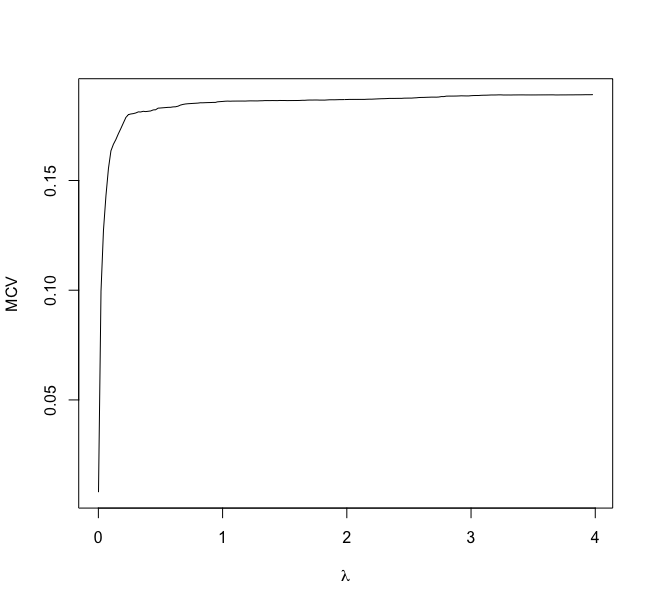
\includegraphics[width=0.5\linewidth]{MCVfail}
\centering
\caption{MCV($\lambda$) for one of the binned data sets (as in line~\ref{blah2} of algorithm~\ref{BLB}) when performing BLB on the same data set as shown in Figure \ref{fig:edf}, with $b=333$ and $s=15$ so that $b\times s\approx 5000$. We can see that the MCV function attains its minimum at $\lambda=0$ implying no smoothing. 
%Note that each BLB binned data set, despite having nominal size 5,000, contains at most 333 distinct points. 
}
\label{fig:badMCV}
\end{figure}

In general, the problem illustrated with the previous toy example also occurs in larger datasets. If we take $b=n^{\gamma}$ where $\gamma\in [0.5,1]$ as recommended by \citet{kleiner2014scalable}, the number of repeats for each distinct point in the bootstrap sample should be around $n/b=n^{1-\gamma}$. As long as there is one point in the testing set that is outside of the convex hull, we would lose at least $n^{1-\gamma}$ validation points, which is a significant amount when $n$ is large. Also, when calculating the MCV statistic, we are only fitting models for training sets that are portions of the original data set of interest. It is not clear whether the optimum $\lambda^*$ we obtain is best for the individual training subsets, or for the original data set that has larger sample size and more variable data.

We therefore propose a new Cross-Validation for Binned data sets (CVB) statistic, a different way of selecting the smoothing parameter $\lambda$ that is easy to optimize, works properly with BLB binned data, and finds the best smoothing constant by considering all information from the original data set. Following the steps of BLB, we first randomly generate $s$ disjoint subsamples of size $b$. We resample each subsample once to get $s$ binned data sets, $\mathbb{H}_1,\cdots,\mathbb{H}_s$, each with nominal size $n$. For each proposed $\lambda$ value, we ``loop around" by  fitting the quantile smoothing splines with one of the binned data sets and predict on the next full-size sample to calculate the prediction score. The convex hull of each of the $s$ data sets will be approximately equal, given they were obtained randomly and they do not overlap, hence few validation points will be lost. We take an average of the errors across the $s$ samples, and obtain the new criterion
\begin{equation}
\label{MCVB}
    \mbox{CVB}(\lambda)=\frac{1}{s}\sum_{j=1}^{s} \frac{1}{|\mathbb{H}_{j+1}|}\sum_{(x_i,y_i)\in \mathbb{H}_{j+1}} \rho_{\tau}[y_i-\hat{g}_{\lambda}^{[\mathbb{H}_j]}(x_i)],
\end{equation}
where $\mathbb{H}_{s+1}=\mathbb{H}_1$, and $\hat{g}_{\lambda}^{[\mathbb{H}_j]}$ denotes the smoothing spline fitted to the full-sized $\mathbb{H}_j$ and $|\mathbb{H}_{j+1}|$ is the number of $(x_i,y_i)$ data points in $\mathbb{H}_{j+1}$. 

Note that we treat the binned data sets obtained from the subsamples as if they were the different folds when calculating MCV in \eqref{MCV}. This procedure utilizes a distributed computing architecture and can be integrated into the BLB algorithm. Also, we are fitting the quantile smoothing splines with different $\lambda$ values to BLB binned data sets. Since the subsamples are disjoint with each other, we will not have the problem of zero prediction scores. Moreover, the parameter selected can be used for every bootstrap sample generated from different subsamples. The optimum smoothing parameter $\lambda^*$ obtained via minimizing \eqref{MCVB} clearly suits our purpose better than other alternatives, and hence we use $\lambda^*$ as the smoothing parameter in each bootstrap run. Figure \ref{fig:diagram} illustrates how to incorporate $\text{CVB}(\lambda)$ into BLB and explains the structural design of our full method. Detailed information of the BLB-CVB method is given in Algorithm \ref{fullmodel}. 
\begin{figure}[H]
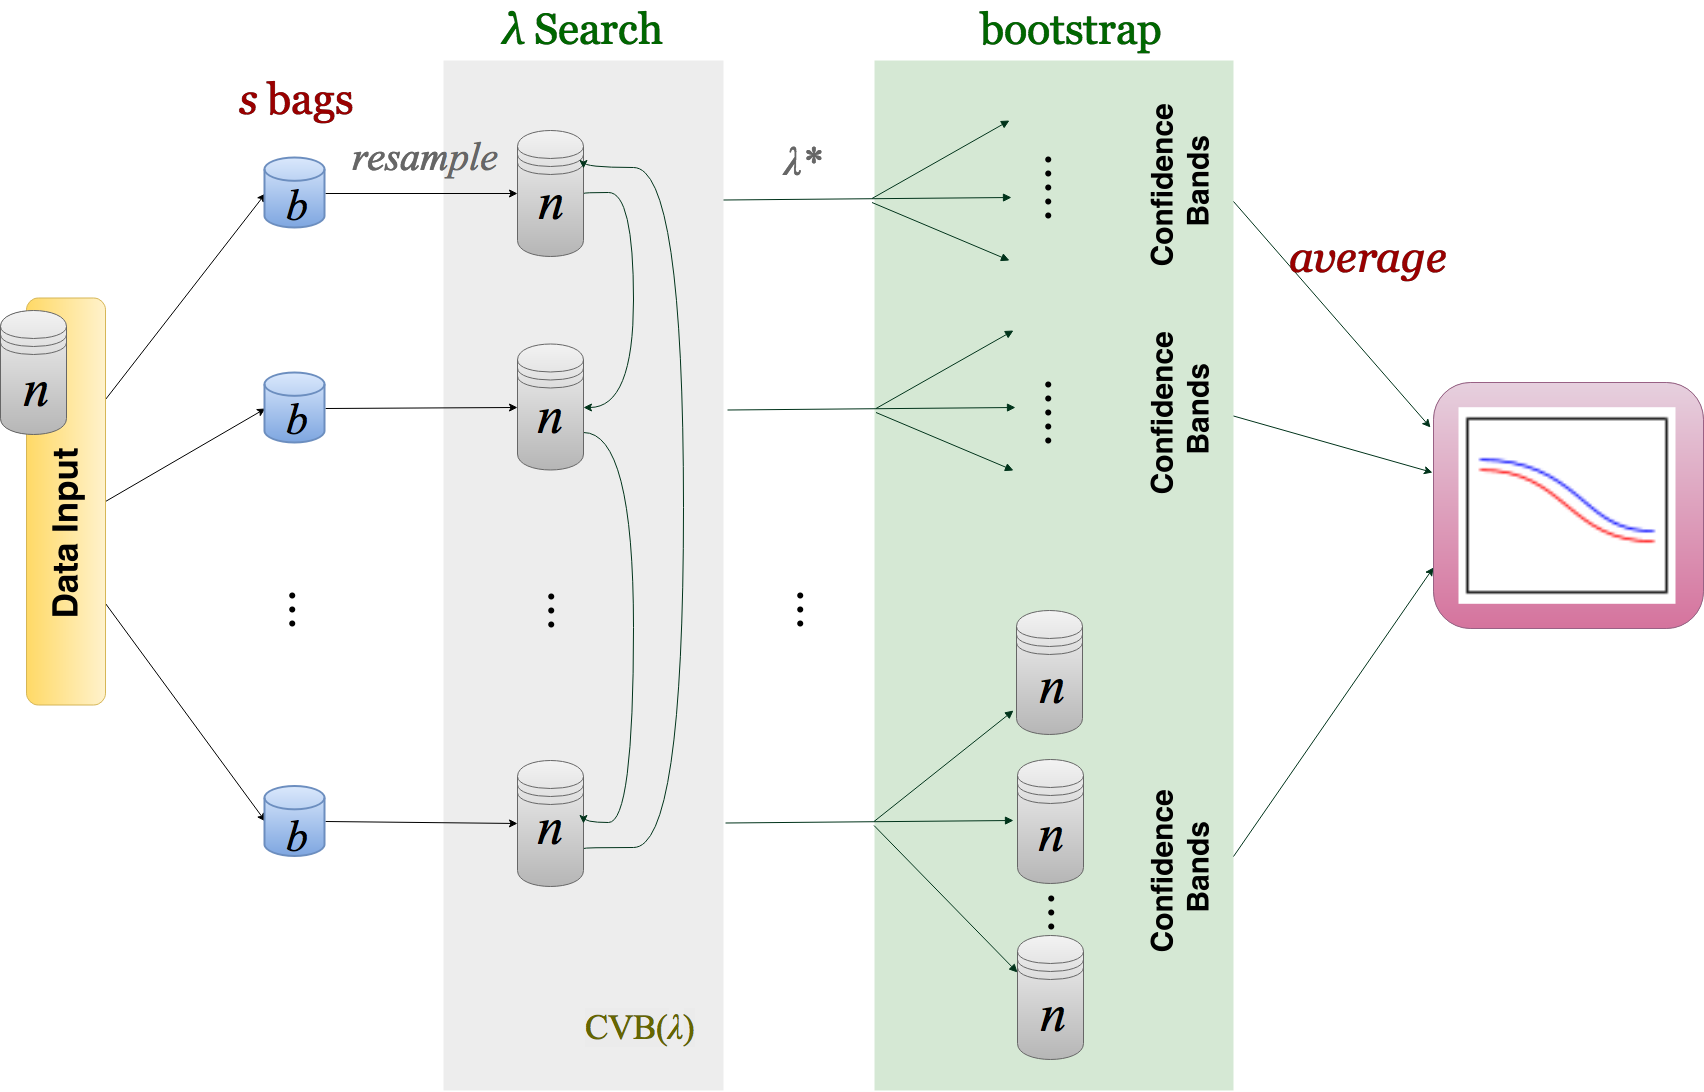
\includegraphics[width=0.9\linewidth]{diagram}
\centering
\caption{A schematic diagram of the BLB-CVB methodology. The optimum parameter $\lambda^*$ is obtained prior to bootstrapping by optimizing the CVB($\lambda$) criterion, which relies on cross-validation of the binned data, achieving the speed-up advantages of BLB. The confidence bands are obtained by averaging the bands obtained from each `bag'.}
\label{fig:diagram}
\end{figure}

Figure \ref{fig:blb5000} displays the $\text{CVB}(\lambda)$ function for the BLB binned data sets generated from the same data set as shown in Figure \ref{fig:edf}. The new metric is well-behaved (smooth) and easy to optimize. After choosing the minima of $\text{CVB}(\lambda)$ as our $\lambda^*$, we ran the bootstrap $r=100$ times for each subsample and obtain a pointwise 95\% confidence bands for the median over a uniformly distributed sequence on $[-1,1]$ with length $200$. The results are plotted in the right panel of Figure \ref{fig:blb5000}. We can see that the true median curve lies within our confidence bands almost everywhere (Section \ref{s5} presents  a comprehensive coverage analysis). A real-life application of our method to compare two scenarios in very large climate data sets (section \ref{USA}) indicates $\text{CVB}(\lambda)$ is a smooth function and exhibits convexity for data sets with larger size. The $\text{CVB}(\lambda)$ curve becomes flatter when the smoothing parameter grows extremely large. 

\begin{algorithm}[H]
\caption{BLB for confidence bands on quantile smoothing splines using  CVB$(\lambda)$}\label{fullmodel}
\begin{algorithmic}[1]
\Require \begin{tabular}{ll}
     Data $\mathbb{X}=\{(\mathbf{x}_i,y_i);i=1,\cdots,n\}$\qquad\qquad&$b$: size of subsets or `bags'\\
    $\tau$: quantile of interest&$s$: number of subsets or `bags'\\
   $\alpha$: significance level&$r$: number of bootstraps of each subset\\
   &$\mathcal{L}$: a sequence of $\lambda$ candidate values
\end{tabular}
\Ensure  CVB values over $\mathcal{L}$ and $\lambda^*$ that minimizes CVB
\Statex \qquad\;\; Estimated confidence intervals for the $\tau$th quantile function

   \State Shuffle $\{1,\cdots,n\}$ and partition the set into disjoint subsets of size $b$ 
   \State Choose the first $s$ subsets: $\mathcal{I}_1,\cdots,\mathcal{I}_s$
   \State Sample $s$ weight vectors where $(w_1^{(j)},\cdots,w_b^{(j)})\sim \text{Multinomial}(n,\mathbf{1}_b/b),\text{ }j=1,\cdots,s$
   \For {$j \leftarrow 1, s$}\Comment{Calculate $\text{CVB}(\lambda)$}
        \If{$j==s$} $j^*\leftarrow 1$ 
        \Else $\text{ }j^*\leftarrow j+1$
        \EndIf
      \State Generate two subsets $\mathbb{B}_1$ and  $\mathbb{B}_2$ by subsetting $\mathbb{X}$ using indices $\mathcal{I}_j$ and $\mathcal{I}_{j^*}$ respectively
      \State Obtain BLB binned samples: 
      \Statex \; $\mathbb{H}_1=\{\mathbb{B}_1\text{ weighted by }(w_1^{(j)},\cdots,w_b^{(j)})\}$ and $\mathbb{H}_2=\{\mathbb{B}_2\text{ weighted by }(w_1^{(j^*)},\cdots,w_b^{(j^*)})\}$
      \For {$\lambda\in\mathcal{L}$}
        \State Fit quantile smoothing splines on $\mathbb{H}_1$ and get the $\tau$th quantile function $\hat{g}_{\lambda}^{[\mathbb{H}_1]}$
        \State Predict on $\mathbb{H}_2$ to get the prediction score: $\sum_{(x_i,y_i)\in \mathbb{H}_2} \rho_{\tau}[y_i-\hat{g}_{\lambda}^{[\mathbb{H}_1]}(x_i)]$
        \State Save the score to {\tt Score}[j,$\lambda$]
      \EndFor
   \EndFor
   \State Average the results and get: $\text{CVB}(\lambda)=\frac{1}{s}\sum_{j=1}^s${\tt Score}[j,$\lambda$] where $\lambda \in \mathcal{L}$
   \State $\lambda^*\leftarrow\lambda$ that minimizes $\text{CVB}(\lambda)$
   \For {$j \leftarrow 1, s$}\Comment{Bootstrapping}
      \State Generate a subset or `bag' $\mathbb{B}$ by subsetting $\mathbb{X}$ using indices $\mathcal{I}_j$
      \For {$k \leftarrow 1, r$}
         \State Sample $(w_1,\cdots,w_b)\sim \text{Multinomial}(n,\mathbf{1}_b/b)$ 
         \State Obtain the bootstrap sample: $\mathbb{H}=\{\mathbb{B}\text{ weighted by }(w_1,\cdots,w_b)\}$
         \State Fit $\tau$th quantile smoothing splines on $\mathbb{H}$ with $\lambda^*$
      \EndFor
      \State Calculate $(1-\alpha)$\% empirical confidence bands $(L_j,U_j)$ for the quantile function
   \EndFor
   \State $(L,U) \leftarrow \frac{1}{s}\sum_{j=1}^s{(L_j,U_j)}$ \Comment{Average the $s$ confidence bands}
\end{algorithmic}
\end{algorithm}

\begin{figure}[H]
\centering   
  \subfigure[$\lambda^*=6.4,\text{CVB}(\lambda^*)=0.20010$]{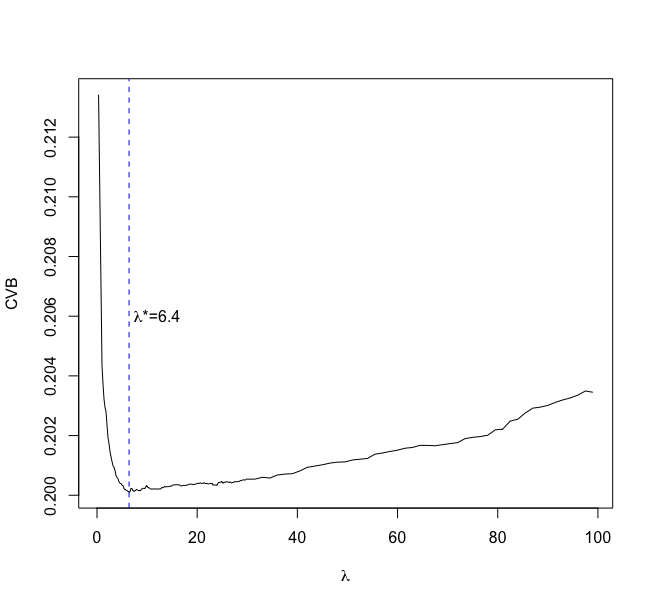
\includegraphics[width=70mm]{CVB.png}}
  \subfigure[Median confidence bands ($\alpha=0.05$)]{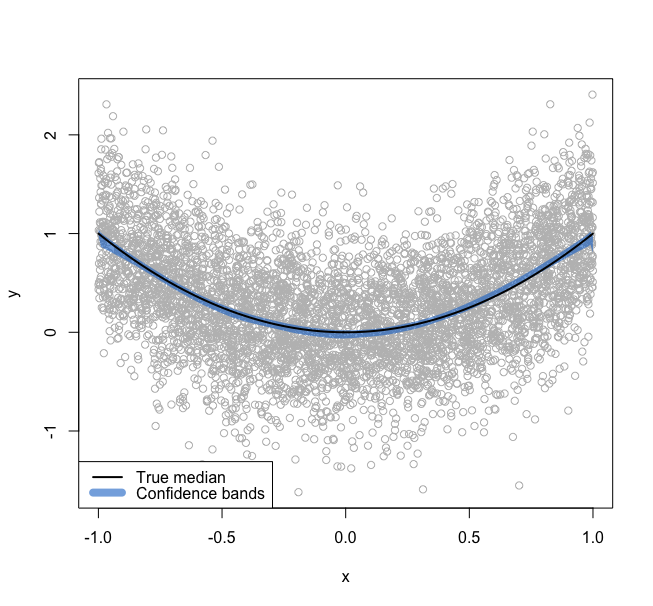
\includegraphics[width=70mm]{CB.png}}
\caption{For the same data set as shown in figure \ref{fig:edf}, we follow the procedure in figure \ref{fig:diagram} and calculate the CVB function to select an optimum parameter and then run the bootstrap. Again, the parameters for BLB are set to be: $b=333, s=15, r=100$. In the right panel, we showed the pointwise 95\% confidence bands for the median over a uniformly distributed grid on $[-1,1]$.}
\label{fig:blb5000}
\end{figure}

In summary, CVB is a robust, reliable, and computationally efficient means of assessing the trade-off between fidelity and smoothness and for automatically selecting the optimum smoothing parameter. 

\section{Performance analysis of the BLB-CVB method}\label{s5}

In this section we study the coverage properties of bootstrapped confidence bands (i.e., for quantile functions of one regressor) and confidence surfaces (i.e., quantile functions of two regressors) derived using the approach described in sections \ref{s3} and \ref{lambdasel}. We also report on the computational costs of the procedures.

\subsection{Coverage analysis for univariate quantile smoothing}

Simulated data sets were generated under four different models. For each model, we simulated $200$ data sets each consisting of $50,000$ observations. For each data set, we ran the complete BLB analysis with automatic $\lambda$ search and confidence bands computation. We set $b=3333$, $s=15$ so that $b*s/n=99.9\%$ and practically all information is utilized in the bootstrapping process; we use $r=100$ in all runs of BLB. The four true underlying models are (see Figure \ref{fig:sim}):
\begin{itemize}
    \item \textbf{Model I:} $y=x^2+\epsilon, \quad \epsilon\sim N(0,0.5^2)$,
    \item \textbf{Model II:} $y=sin(\pi x)+\epsilon, \quad \epsilon\sim t_3$,
    \item \textbf{Model III:} $y=x^2+\epsilon, \quad \epsilon\sim 0.45N(0,1)+0.55N(3,1)$,
    \item \textbf{Model IV:} $y=1+x+x^2\epsilon, \quad \epsilon\sim N(0,0.5^2) $.
\end{itemize}
To evaluate the confidence interval and surface estimates,  we follow standard coverage simulation practice, computing the coverage rate as the proportion of times the true function value at each $x$ is contained within the bootstrap intervals.  In every case presented in this section, the nominal confidence level was $0.95$ ($\alpha=0.05$). Coverage rates were computed in a pointwise manner for a set of $x$ values in the $(-1,1)$ interval.
\begin{figure}
\centering   
  \subfigure[Model I]{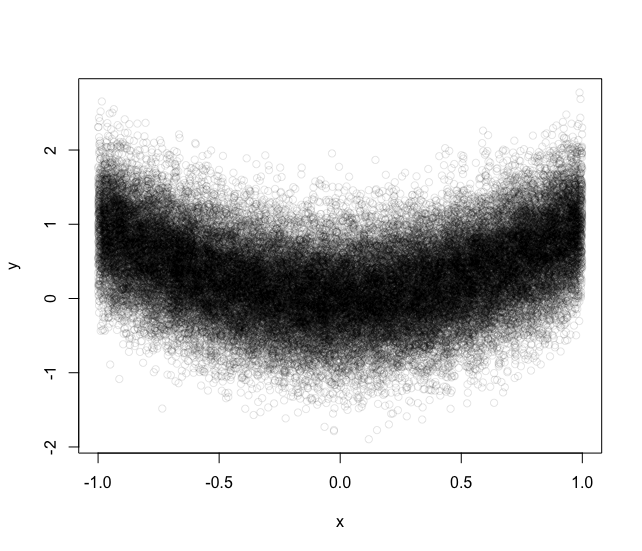
\includegraphics[width=70mm]{model1.png}}
  \subfigure[Model II]{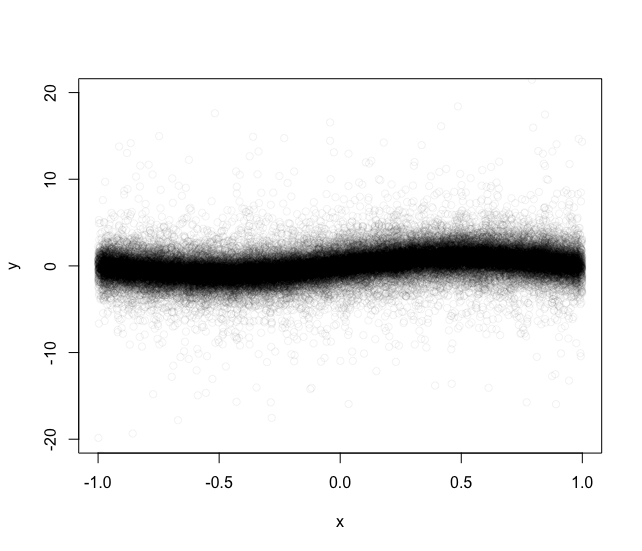
\includegraphics[width=70mm]{model2.png}}
  \subfigure[Model III]{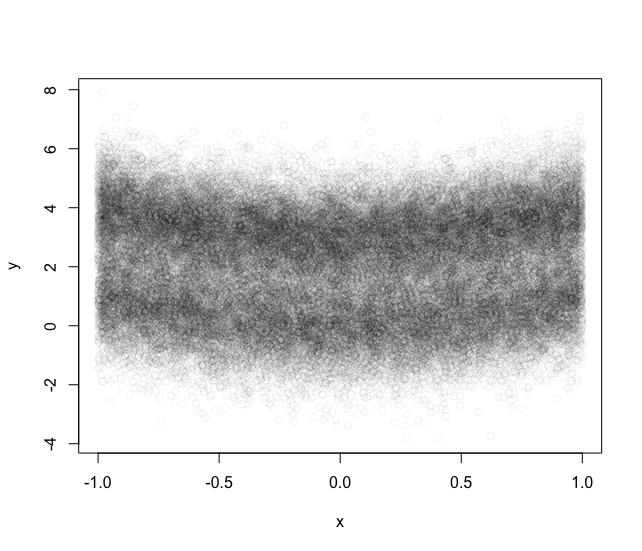
\includegraphics[width=70mm]{model3.png}}
  \subfigure[Model IV]{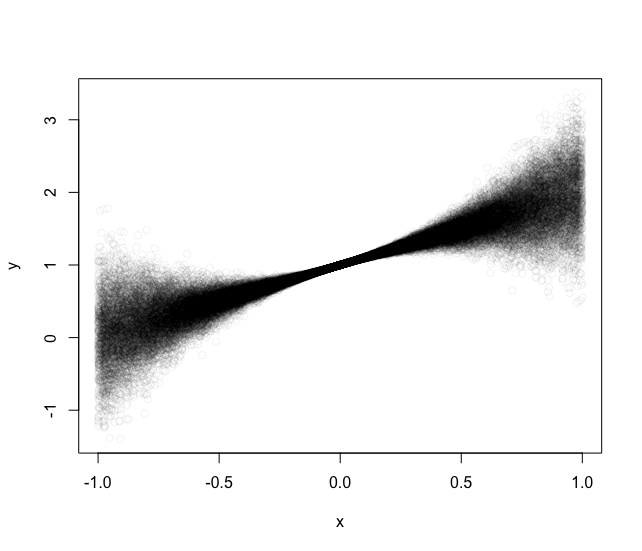
\includegraphics[width=70mm]{model4.png}}
\caption{50,000 observations simulated from each of four models.}
    \label{fig:sim}
\end{figure}

\subsubsection{Results for the four simulated models}
\begin{figure}
\centering   
  \subfigure[\textbf{Model I, $\tau=0.5$}]{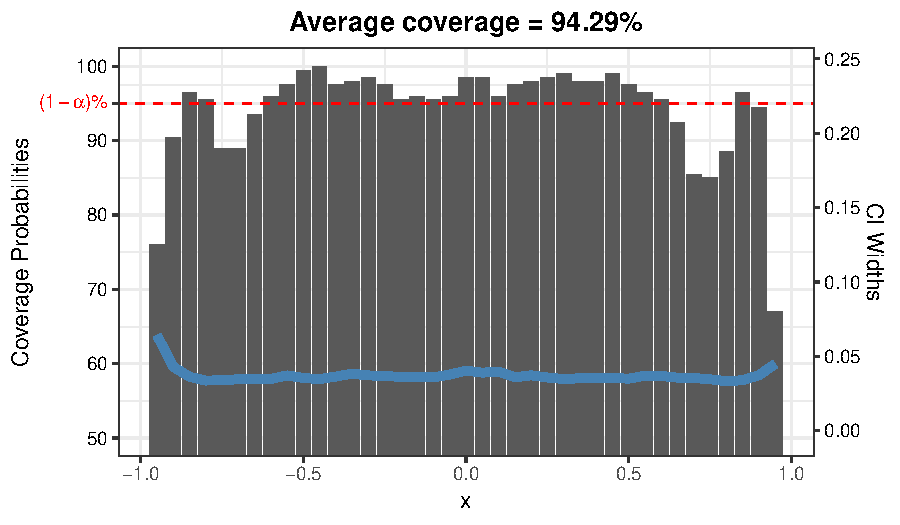
\includegraphics[width=70mm]{m11.pdf}}
  \subfigure[\textbf{Model I, $\tau=0.95$}]{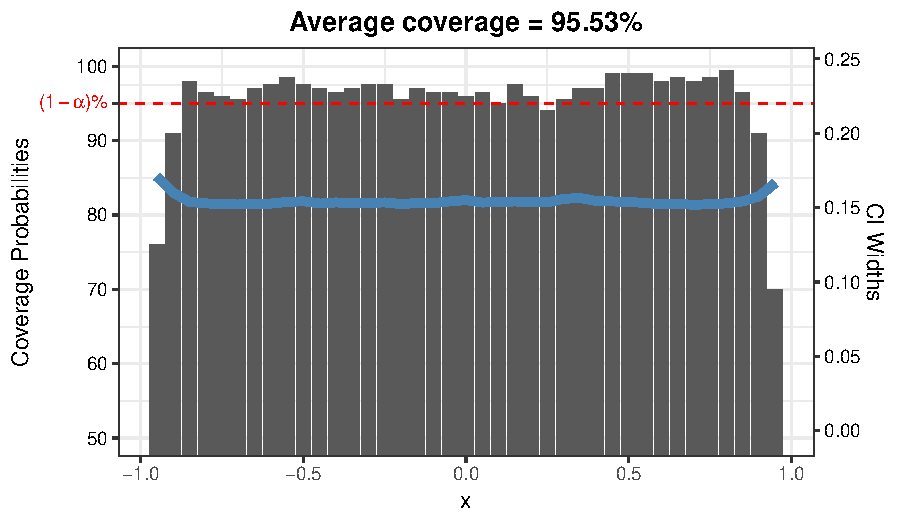
\includegraphics[width=70mm]{m12.pdf}}
  
  \subfigure[\textbf{Model II, $\tau=0.5$}]{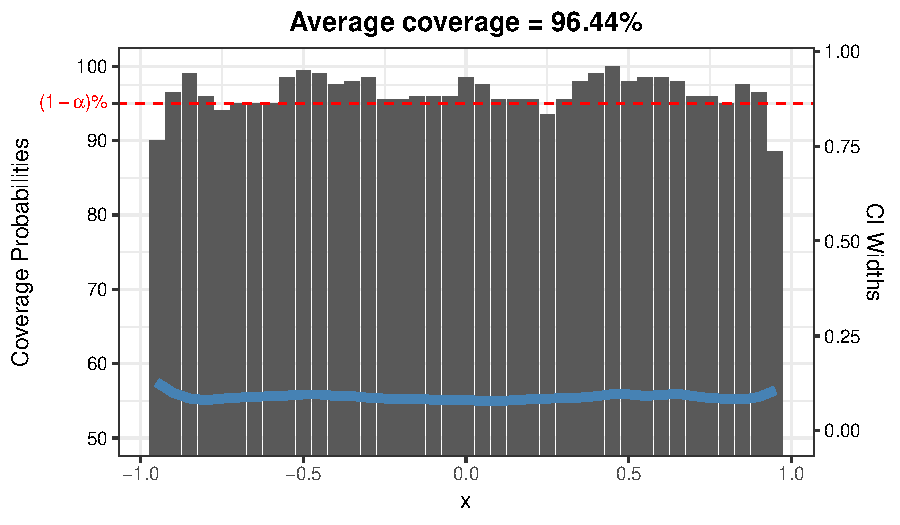
\includegraphics[width=70mm]{m21.pdf}}
  \subfigure[\textbf{Model II, $\tau=0.95$}]{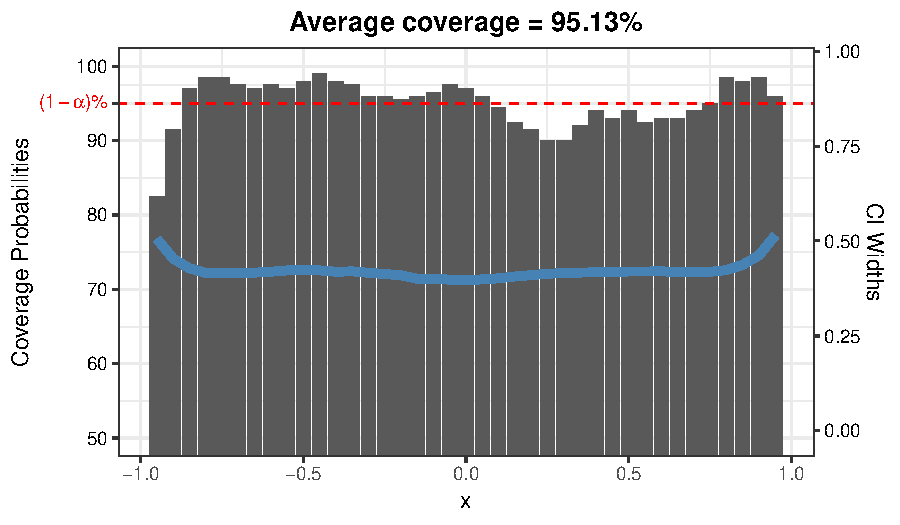
\includegraphics[width=70mm]{m22.pdf}}
  
  \subfigure[\textbf{Model III, $\tau=0.5$}]{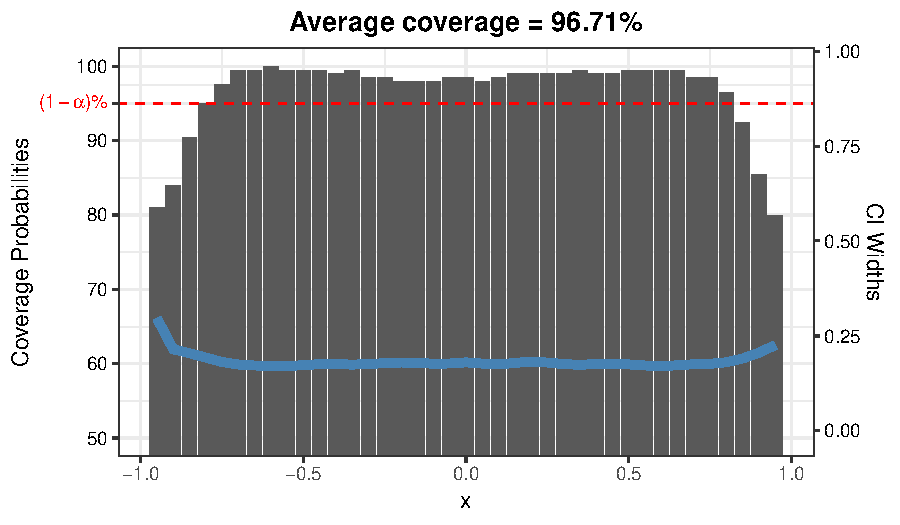
\includegraphics[width=70mm]{m31.pdf}}
  \subfigure[\textbf{Model III, $\tau=0.95$}]{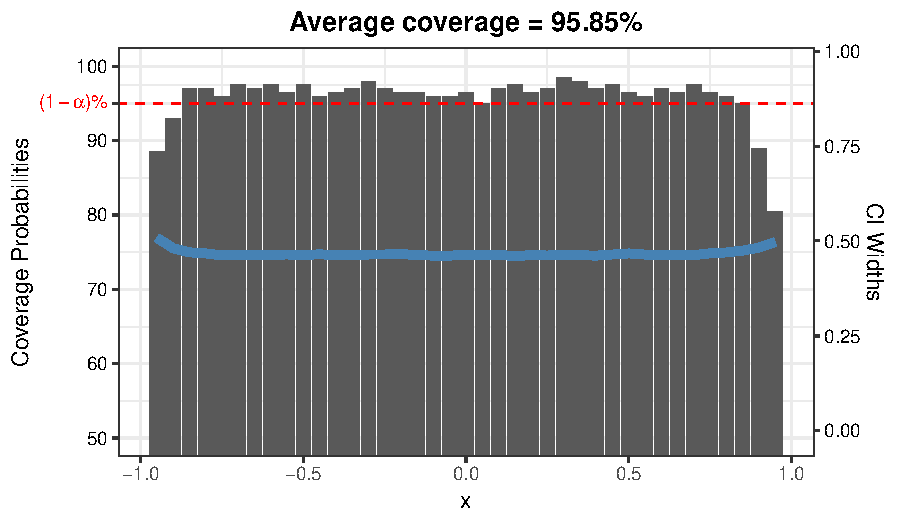
\includegraphics[width=70mm]{m32.pdf}}
  
  \subfigure[\textbf{Model IV, $\tau=0.5$}]{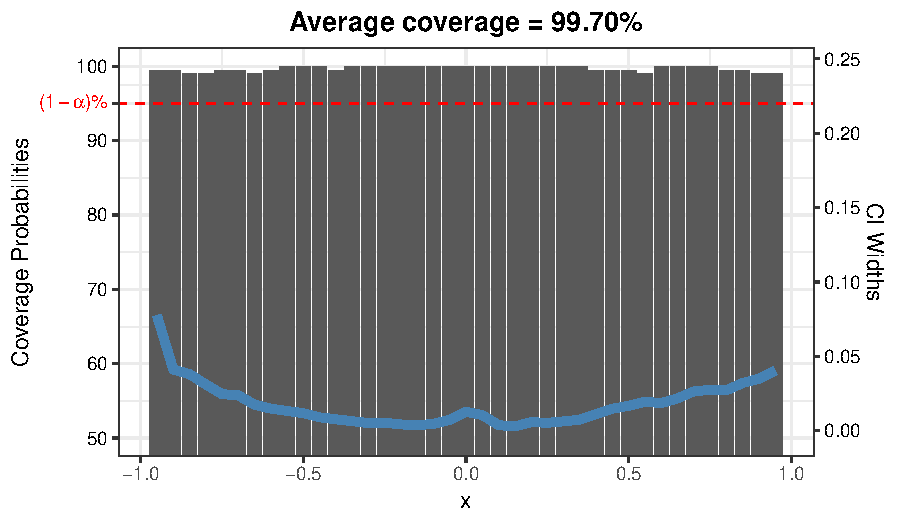
\includegraphics[width=70mm]{m41.pdf}}
  \subfigure[\textbf{Model IV, $\tau=0.95$}]{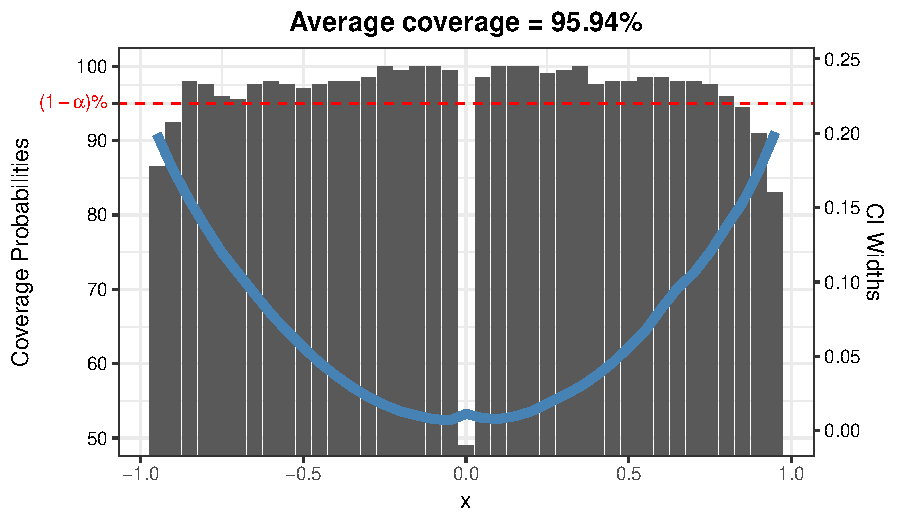
\includegraphics[width=70mm]{m42.pdf}}
\caption{Coverage probabilities (in histograms) and average CI widths (in blues lines) for the four different models at $\tau=0.5$ (a, c, e, g) and $\tau=0.95$ (b, d, f, h).}
\label{fig:coverProb}
\end{figure}
The results from the coverage analyses are displayed as histograms in Figure \ref{fig:coverProb}. We can see that the coverage probabilities of the pointwise intervals are mostly near the advertised $(1-\alpha)\%$ level while the CI widths are consistently a small fraction of the y-range of the data sets. We observe an edge effect, as the CIs generally feature poorer performance at the boundaries of the domain. This is because the bulk of the data is located in the middle of the domain, driving the smoothness of the fitted quantile function. There is just not enough information for the function to change the curvature  {near the edges. Also, seeing that each `bag' may not cover the entire domain, mild extrapolation may still result from the BLB-CVB fitting procedure near the boundaries, leading to poor coverage rates.}   {We also observe that the confidence bands are narrower for $\tau=0.5$ as compared with $\tau=0.95$, though the coverage rates are similar in both cases;  as expected,} results show that it is more difficult to perform inference for extreme quantiles.

\begin{figure}
\begin{center}
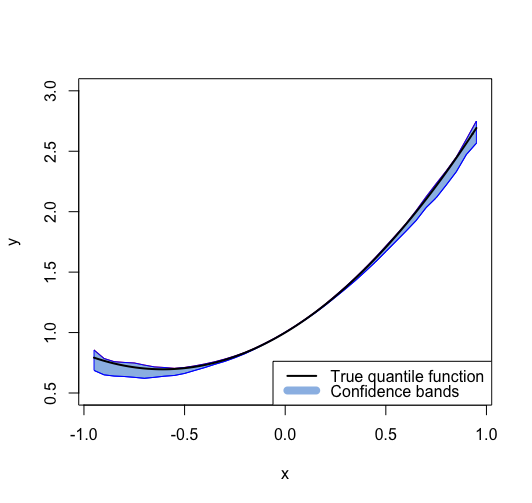
\includegraphics[width=2.5in]{mod4}
\caption{The confidence bands from one of 200 BLB runs for model IV, $\tau=0.95$.}
\label{mod4}
\end{center}
\end{figure}
An interesting feature is that for model IV, $\tau=0.95$, the coverage probability for $x=0$, which is the bottleneck of the vase-shaped data set, is lower than those probabilities for other $x$-values. Figure \ref{mod4} shows the confidence bands from one of 200 BLB runs. Note that the variance of the error term $x^2\epsilon$ decreases to 0 as $x\rightarrow 0$, and thus the quantile function at $x=0$ will be a constant of 1 on $\tau\in (0,1)$. As a result, the width of the bands become narrower around the center of the domain ($0.0035$ when $x=0$). Although the bands are still very close to the true quantile ($<0.003$ difference), they often fail to include it. This case is rather pathological, and there is little practical impact of missing the 95th percentile in this case.

\subsubsection{The effect of $b \cdot s/n$}

As stated before, we need $b\cdot s\approx n$ to maintain higher-order correctness. Nonetheless, \citet{kleiner2014scalable} suggest that fairly modest values of $b$ and $s$ will be sufficient for the BLB to reach convergence with comparably high accuracy: in regression settings, $s$ values of about $1\sim 2$ suffice for $b=n^{0.9}$ and $s$ values of $10\sim 14$ suffice for $b=n^{0.5}$; in a  classification setting, BLB provides comparable relative error to that of the bootstrap when $b>n^{0.6}$. Note that the product $b \cdot s/n$ equals the proportion of data points used in the BLB process. To see how changing this ratio will affect the performance of BLB for quantile regression, we fix $s=15$ and choose $b$ from $\{n^{0.5},n^{0.7},\lfloor n/s\rfloor \}$ so that, with $n=50,000$, $b \cdot s/n=6.7\%,$  $58.3\%$ and $99.9\%$, respectively. 

\begin{table}
%% Caption MUST come immediately after \begin{table}
\hskip -0.5cm\caption{\label{ratio}Estimated pointwise coverage probabilities for the median ($\tau=0.5$) of model I at selected $x$ values when applying regular bootstrapping and when applying the BLB-CVB method with different values of $b \cdot s/n$ on 200 data sets.
}
\hskip -0.8cm
\begin{tabular}{|l|c|c|c|c|c|c|c|c|c|}
\hline
\cellcolor{Gray} 
$x$            & \cellcolor{Gray} -0.9 &\cellcolor{Gray}  -0.8 & \cellcolor{Gray} -0.7 & \cellcolor{Gray} -0.6 &\cellcolor{Gray}  -0.5 & \cellcolor{Gray} -0.4 &\cellcolor{Gray}  -0.3 &\cellcolor{Gray} -0.2 & \cellcolor{Gray} -0.1 \\ \hline
BLB, $b \cdot s/n=6.7\%$    & 0.530 & 0.480  & 0.405 & 0.425   & 0.425   & 0.470 & 0.495 & 0.455   &0.455\\ \hline
BLB, $b \cdot s/n=58.3\%$   &0.780 & 0.825&   0.740  &   0.810 &   0.925& 0.925 &0.880  &  0.895  &0.915\\ \hline
BLB, $b \cdot s/n=99.9\%$ & 0.930   & 0.935   & 0.900 & 0.955 & 0.995 & 0.980 & 0.980   & 0.970 &0.975\\ \hline
bootstrap, $r=200$ & 0.955   & 0.965   & 0.970 & 0.960 & 0.955 & 0.965 & 0.960   & 0.985 &0.970\\ \hline
\cellcolor{Gray}  
$x$            &\cellcolor{Gray}  0.1 & \cellcolor{Gray} 0.2 &\cellcolor{Gray}  0.3 &\cellcolor{Gray} 0.4 & \cellcolor{Gray} 0.5 & \cellcolor{Gray} 0.6 & \cellcolor{Gray} 0.7 & \cellcolor{Gray} 0.8 & \cellcolor{Gray} 0.9\\ \hline
BLB, $b \cdot s/n=6.7\%$    & 0.435 & 0.440   & 0.450 & 0.390   & 0.435   & 0.470& 0.425 & 0.465  & 0.455\\ \hline
BLB, $b \cdot s/n=58.3\%$  & 0.905 & 0.910 & 0.910  & 0.865 &  0.885  &  0.765  & 0.720 & 0.775 &  0.800  \\ \hline
BLB, $b \cdot s/n=99.9\%$  & 0.970   & 0.965   & 0.985 & 0.995 & 0.985 & 0.955 & 0.880   & 0.930 &0.955\\ \hline
bootstrap, $r=200$ & 0.965   & 0.940   & 0.970 & 0.960 & 0.945 & 0.945 & 0.970   & 0.960 &0.955\\ \hline
\end{tabular}
\end{table}

\begin{figure}[H]
\caption{Confidence bands  {for Model I} from one BLB run using two different $b \cdot s/n$ ratios.} \label{fig:ratio}
\centering   
  \subfigure[$b \cdot s/n=6.7\%$, $\tau=0.5$]{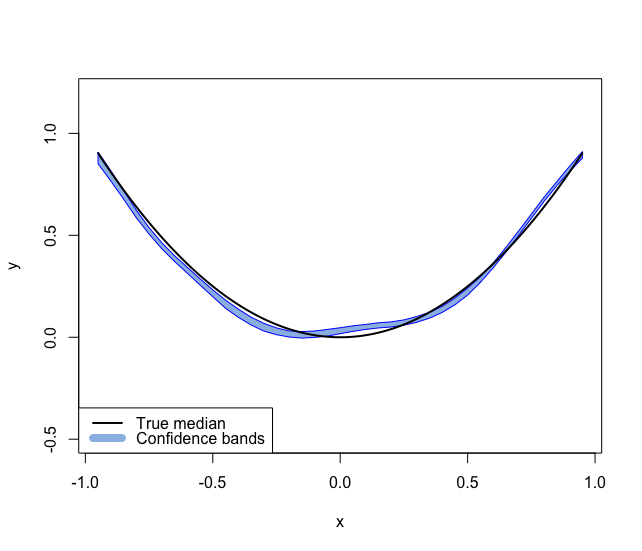
\includegraphics[width=70mm]{6per.png}}
  \subfigure[$b \cdot s/n=99.9\%$, $\tau=0.5$]{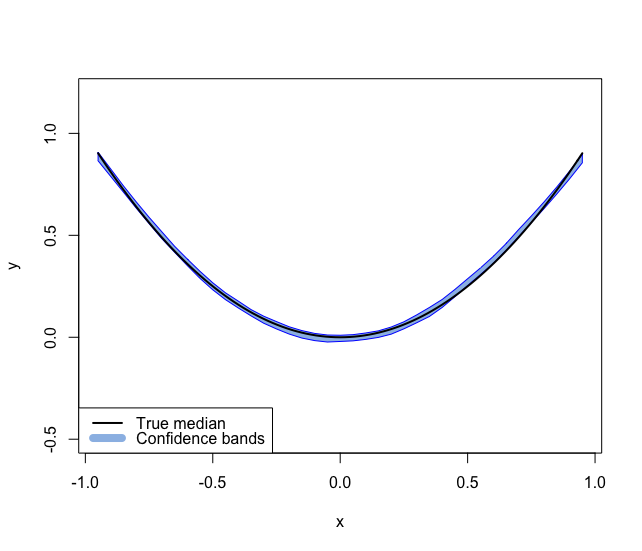
\includegraphics[width=70mm]{93per.png}}
\end{figure}
Table \ref{ratio} shows the coverage probabilities for Model I, derived using the BLB procedure with the three different ratios of $b \cdot s/n$. Increasing the fraction of the original data points that are included in the BLB computation (increasing $b \cdot s/n$) improves the coverage rates. Also, the BLB implementation with $b=n^{0.7}$ displays comparable results to that of the regular bootstrap, in agreement with  the results of Kleiner et al. Figure \ref{fig:ratio} shows how BLB fails to capture the true underlying median function when $b \cdot s/n$ is too small.

\subsubsection{Execution time comparison}
We performed a small scale simulation study to compare the execution time needed to compute confidence bands using both the BLB method and the conventional bootstrap, respectively, for data sets of different sizes. {We only consider 9 data sets generated from model I varying  $n$ from $e^{11}$ to $e^{15}$ in increments of $e^{0.5}$ (note $e^{11}\approx 6\times 10^4$, and $e^{15}\approx 3\times 10^6$). For BLB, the number of `bags' was set to $s=15$, and $b=\lfloor{n^{\gamma}}\rfloor$, where $\gamma=0.5,0.6,0.75$}.  {For both regular bootstrap and bootstrapping within BLB}, the number of resamples was set at $r=100$. Here we want to examine the efficiency of these two methods when computing the confidence bands, and thus we fix the smoothing parameter at $\lambda=2$ and do not perform the MCV (for the bootstrap) or CVB (for the BLB) step. 

The observed running times are reported in Figure \ref{time}. The BLB method clearly improves upon the conventional bootstrap with respect to time savings when $n$ is large. The OLS coefficients from regressing the log of execution time on the log of sample sizes are also reported in the legend of the figure. The estimated slopes are consistent with what was shown in \citet{koenker2005frisch}, and indicate the execution time grows exponentially in $n$ at a rate of nearly 1.01 for the regular bootstrap, and at rates of 0.06, 0.14, 0.59 for BLB, with $\gamma=0.5,\text{ }0.6$, and 0.75, respectively.
\begin{figure}
\begin{center}
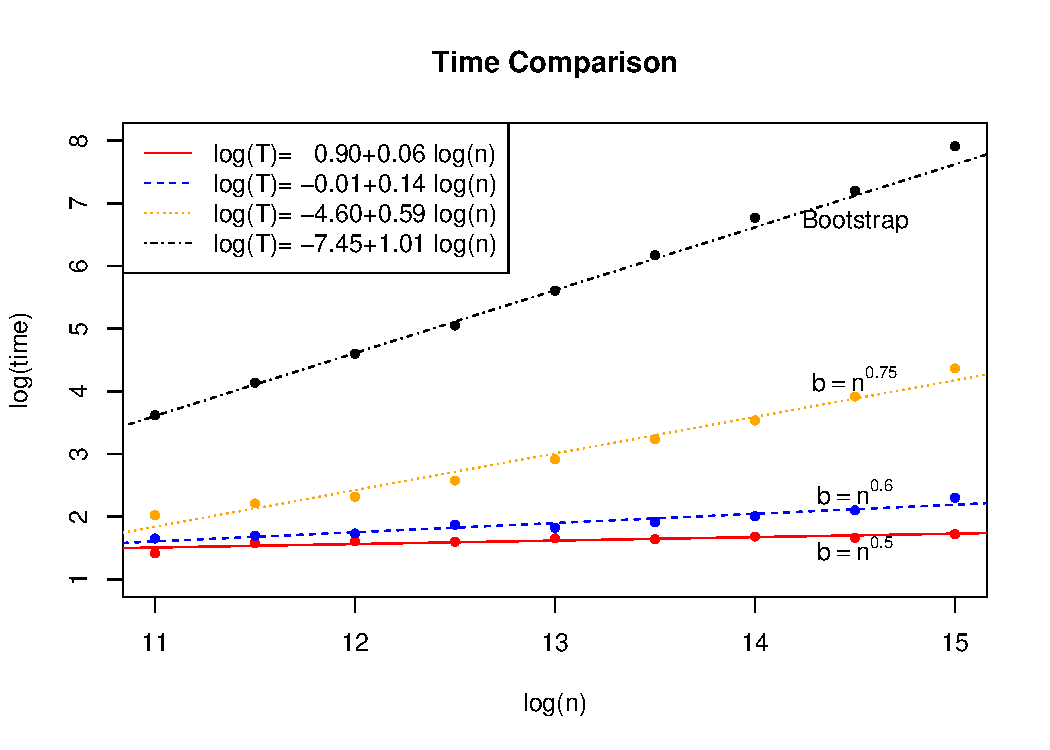
\includegraphics[width=0.6\linewidth]{time.pdf}
\caption{Running time with increasing sample sizes for Model I, $\tau=0.5$.}
\label{time}
\end{center}
\end{figure}

\subsection{Coverage analysis for bivariate quantile smoothing}
To explore the coverage rates of BLB-derived quantile smoothing splines confidence surfaces, two different ``true" surface functions were investigated, each with additive noise. 
\begin{figure}[H]
\centering   
  \subfigure[Sinusoidal ``ridge" surface]{\label{dataShape11}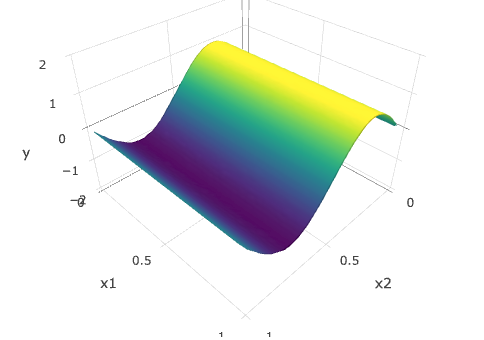
\includegraphics[width=70mm]{RidgePlot.png}}
  \subfigure[Sinusoidal surface of varying frequency]{\label{dataShape12}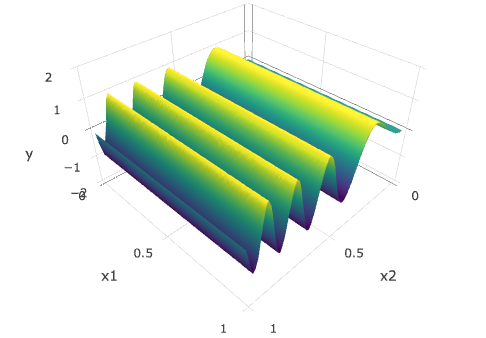
\includegraphics[width=70mm]{CyclesPlot.png}}
  \caption{Two different ``true" surface functions.}
\label{fig:dataShape2}
\end{figure}

The first type of surface tested for coverage analysis is a sinusoidal ``ridge" (see Figure \ref{dataShape11}) with additive $t$-distributed errors:
\begin{equation}
    \label{two1}
    \mathbf{Model\;\;A:\;\;}y_i=\sin(2\pi x_{2i})+\epsilon_i, \text{ where } \epsilon_i\stackrel{iid}{\sim} t_3,\text{ } i=1,\cdots,n,
\end{equation}
where the response does not change along the direction of $x_{1i}$, and $(x_{1i},x_{2i})$ covariates are sampled from independent uniforms on $[0,1]^2$.

The second surface tested for the bivariate coverage analysis is a varying-frequency sinusoidal surface with additive $t_3$ noise (see Figure \ref{dataShape12}):
\begin{equation}
    \label{two2}
    \mathbf{Model\;\;B:\;\;}y_i=x_{1i}+\sin(8\pi x_{2i}^2)+\epsilon_i, \text{ where } \epsilon_i\stackrel{iid}{\sim} t_3,\text{ } i=1,\cdots,n,
\end{equation}
We expect the coverage performance to suffer in this case as, by construction, the smoothness varies over the domain whereas our method assumes spatial stationarity with respect to the smoothing parameter.

Figure \ref{covProb1} shows the estimated pointwise coverage of Model A for the median and 0.95 quantile at a dense grid of points on the unit square $(0,1) \times (0,1)$, based on 200 simulations each with $n=50,000$ observations and the optimal smoothing parameter estimated separately for each simulation. As can be seen, the coverage of the pointwise intervals is adequate throughout the region for both quantiles with slightly lower coverage rates for $\tau=0.95$.
\begin{figure}
\centering   
 {\bf\scriptsize \qquad Average coverage=95.54\%\qquad\quad\qquad\quad\quad\quad Average coverage=93.81\%\qquad\qquad}
 
  \subfigure[Sinusoidal ``ridge" surface]{\label{covProb1}
  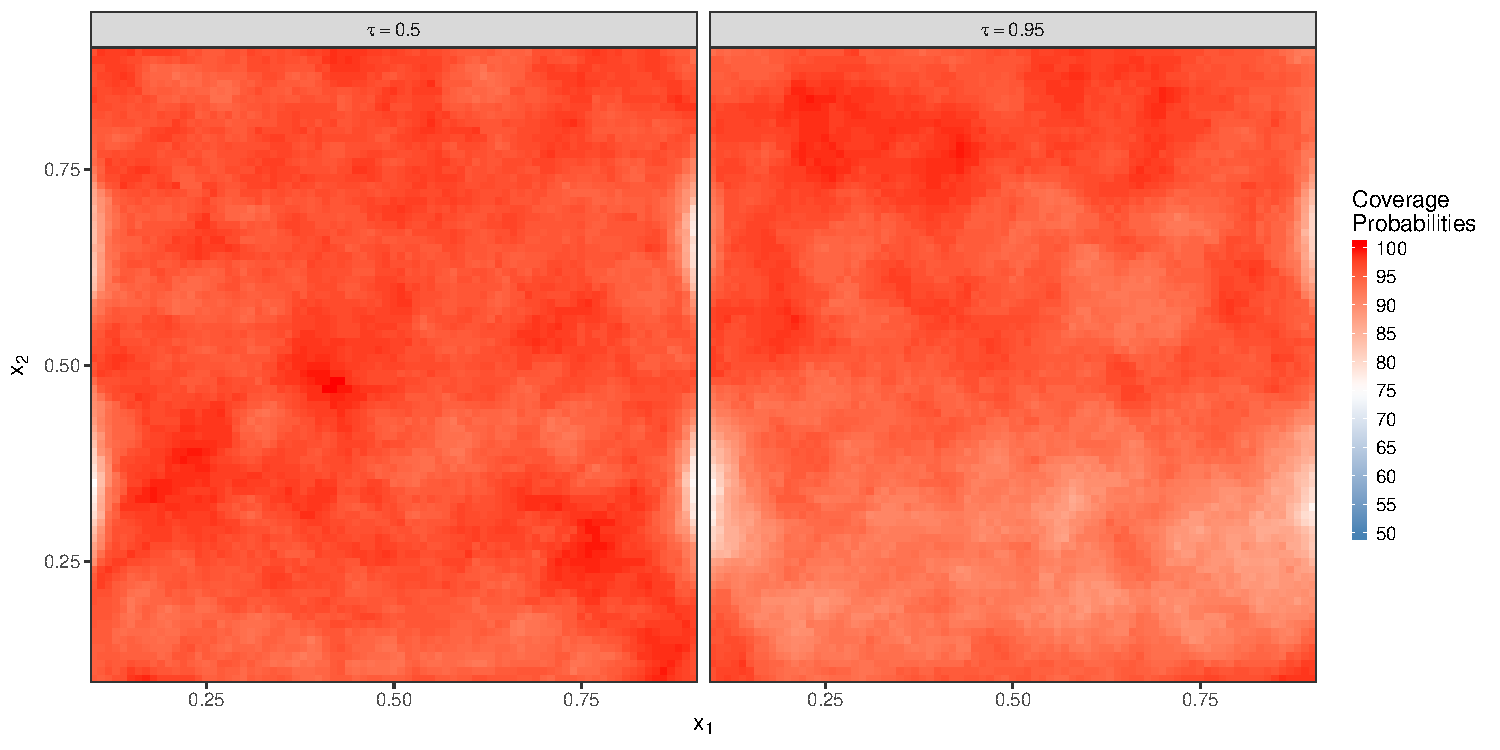
\includegraphics[width=\linewidth,height=0.48\linewidth]{a.pdf}}
 \vskip 0.5cm
 {\bf\scriptsize \qquad Average coverage=95.96\%\qquad\quad\qquad\quad\quad\quad Average coverage=58.02\%\qquad\qquad}
   
  \subfigure[Sinusoidal surface of varying frequency]{\label{covProb2}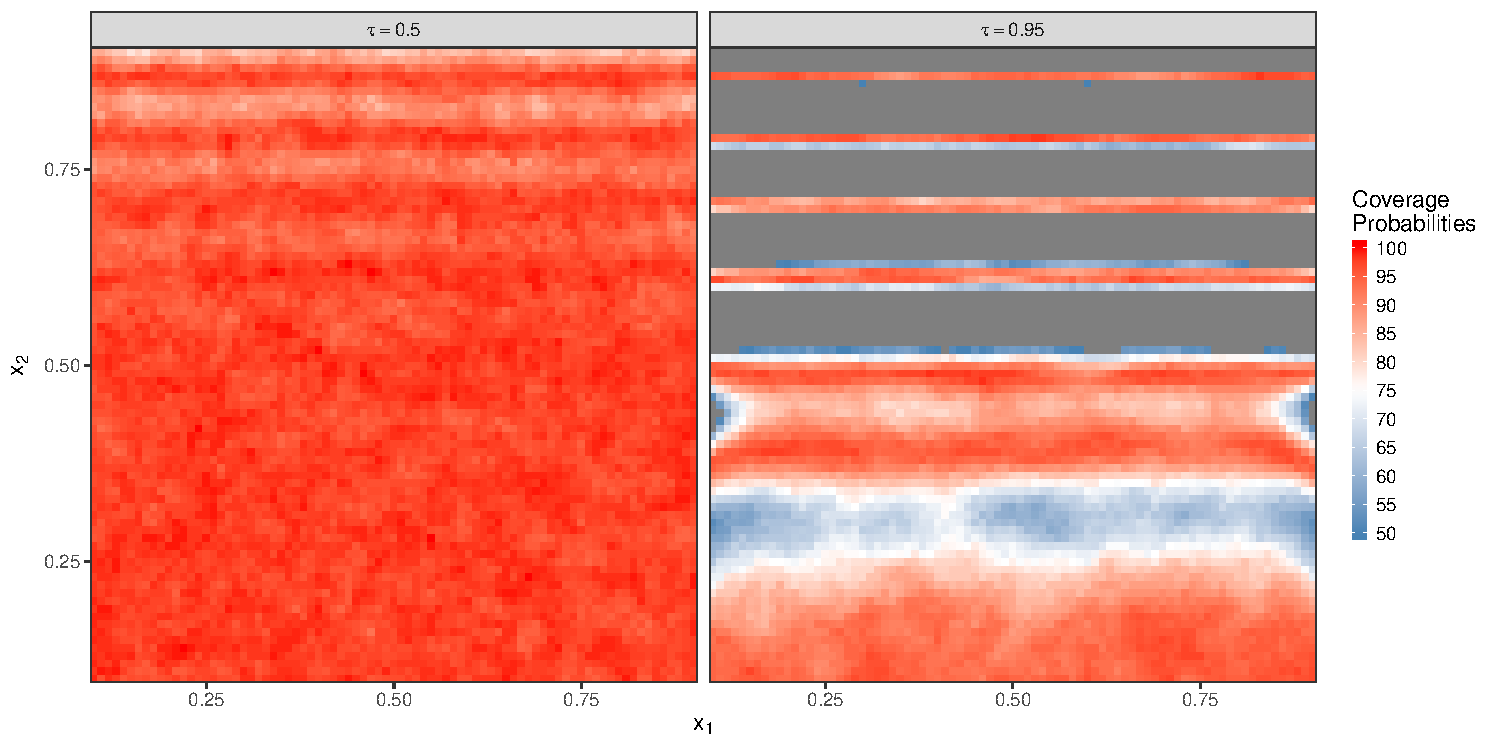
\includegraphics[width=\linewidth,height=0.48\linewidth]{b.pdf}}
\caption{Pointwise coverage probabilities for Model A and Model B.}
\label{fig:covProb}
\end{figure}

In contrast, Figure \ref{covProb2} shows the estimated pointwise coverage rates for Model B. As expected, there are regions in the $x_1-x_2$ plane where the coverage is not adequate, especially where the function oscillates more rapidly, a problem more pronounced for $\tau=0.95$. Here the issue is that the smoothness of the underlying function is not consistent throughout the domain, and therefore it is difficult to select a  {single overall} smoothing parameter that gives accurate quantile estimates over the entire domain.  

In summary, the confidence bands and surfaces for quantile smoothing spline models fitted by our BLB-CVB method exhibit a robust behavior with respect to several functional forms and types of distributional noise, providing close to nominal pointwise coverage  {as long as the stationarity assumption is met.}

\section{An application to NASA's Earth Exchange Climate Data}\label{s6}
We apply the BLB-CVB method for the analysis of comparative experiments via quantile smoothing to the NEX-GDDP data set \citep{thrasher2012bias}. The data set is a global downscaled climate projection ensemble from 21 different climate models at a resolution of $0.25\times 0.25$ degrees ($\sim 25 \text{km}\times 25 \text{km}$). Each of the climate projection data sets includes daily maximum near-surface air temperature, minimum near-surface air temperature, and precipitation for the periods from 1950 through 2005 (retrospective run) and from 2006 to 2100 (prospective run). The predictions are made based on two of the four Representative Concentration Pathways (RCPs) \citep{van2011representative}, representing different carbon dioxide emission and concentration, and land use, trajectories over the 21st century, which were developed for the IPCC's Fifth Assessment Report \citep{IPCCAR5WG1SPM:2013}. 

The two scenarios are RCP 4.5 and RCP 8.5, which correspond to trajectories that would lead to radiative forcing levels of 4.5 and 8.5 $W/m^2$, respectively, by the end of the 21st century\footnote{Radiating forcing is  {a} measure of the amount of energy captured --if positive-- or reflected --if negative-- by the Earth, usually given in Watts per square meter.}. In particular, RCP 4.5 foresees a stabilizing trend of greenhouse gas (especially CO$_2$) emissions and concentrations approximately after 2050. The RCP 8.5 scenario, however, foresees a high population growth and lower rate of technology development, resulting in greenhouse gas emissions that continue to grow over time, leading to higher concentrations and greater radiative forcing \citep{van2011representative}.

The NEX-GDDP data set can be accessed through Amazon's S3 site (\url{s3://nasanex/NEX-GDDP}), and OpenNEX climate data access tools were used to select an area of interest and create a customized data set. Due to its dynamic nature and considerable size, this data set is well-suited to demonstrate the scalability of our methods by considering one possible climate scenario as the ``control" and another scenario the ``treatment" to be compared in time or in space.

\subsection{Comparative experiment with one covariate}
For the one covariate analysis, we use time as the covariate and consider daily maximum temperatures in the Seattle and Chicago areas, respectively, according to one of the 21 models - {\it CCSM4} \citep{gent2011community} under both RCP 4.5 and RCP 8.5. The geographical information on the longitudes and latitudes of the areas of Seattle and Chicago are shown in Figure \ref{fig:Chicago}. Since RCP 8.5 is representative of the high range of non-climate policy scenarios, and RCP 4.5 assumes  a number of climate change mitigating policies scenarios, we treat RCP 8.5 as our ``control" group, and RCP 4.5 as the ``treatment" group. We are interested in comparing how the daily maximum temperature will change under the two different pathways over time in these two cities. 
\begin{figure}
\centering   
  \subfigure{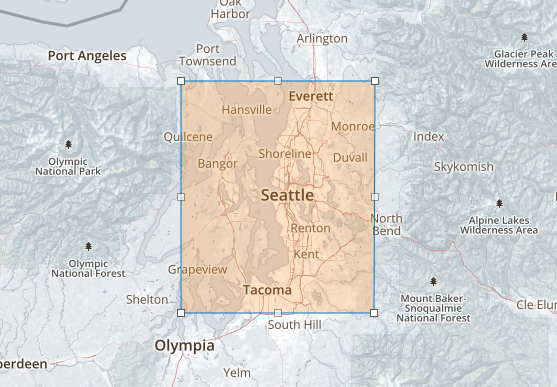
\includegraphics[width=70mm]{Seattle.png}}
  \subfigure{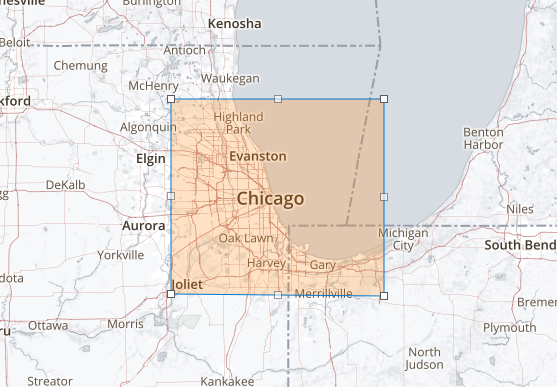
\includegraphics[width=70mm]{Chicago.png}}
\caption{\textbf{Seattle Area} (Lon-Lat): (-122.915, 48.024), (-121.849, 48.024), (-121.855, 47.164), (-122.915, 47.164), (-122.915, 48.024); \textbf{Chicago Area} (Lon-Lat): (-122.915, 48.024), (-121.849, 48.024), (-121.855, 47.164), (-122.915, 47.164), (-122.915, 48.024).}
\label{fig:Chicago}
\end{figure}

To eliminate seasonality from the data, we analyze only the 92 summer days (June to August) for each year from 2006 to 2100 (8740 days in total) and coded the time regressors into $1,2,\cdots, 8740$. For each day, there are 25 down-scaled grid points for each of the Seattle and Chicago areas depicted in Figure \ref{fig:Chicago}. In total there are {\bf 218,500} observations under each RCP scenario. We examine how $\tau=0.5$ and $\tau=0.95$, corresponding to predictions of moderate and extreme summer temperatures respectively, change over time by performing the complete BLB-CVB analysis for both data sets with $s=15$ and $ b=\lfloor n/s\rfloor$. In addition, we take the difference of the quantile estimates between the two scenarios for each bootstrap sample, which yields a set of confidence bands for the differences. 
\begin{figure}
\centering   
  \subfigure[Temperature (\SI{}{\celsius})]{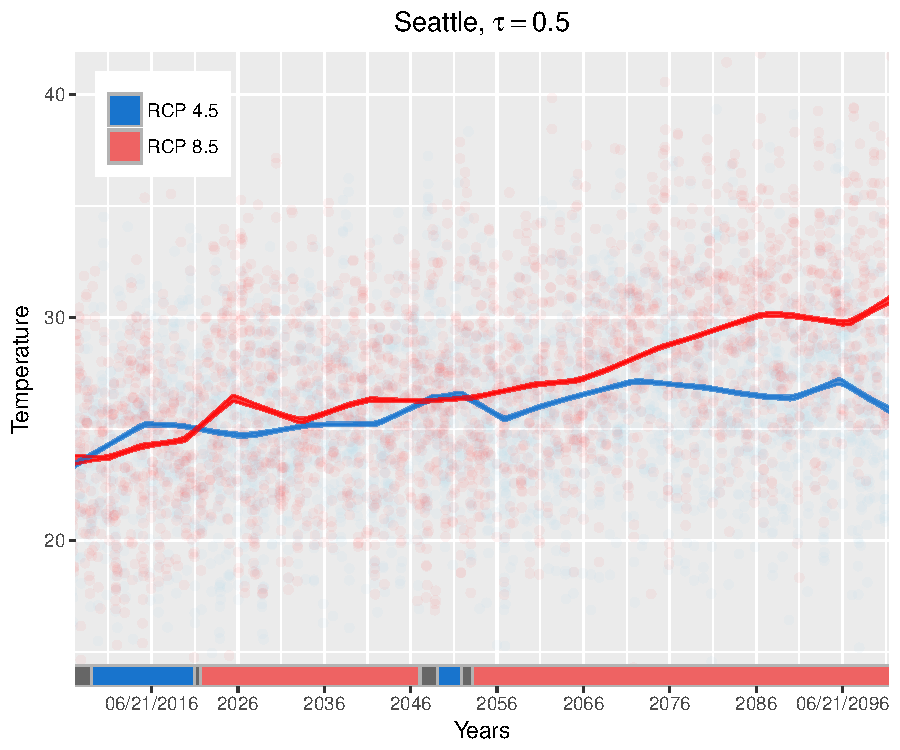
\includegraphics[width=70mm]{T0_5.pdf}}
  \subfigure[Temperature (\SI{}{\celsius})]{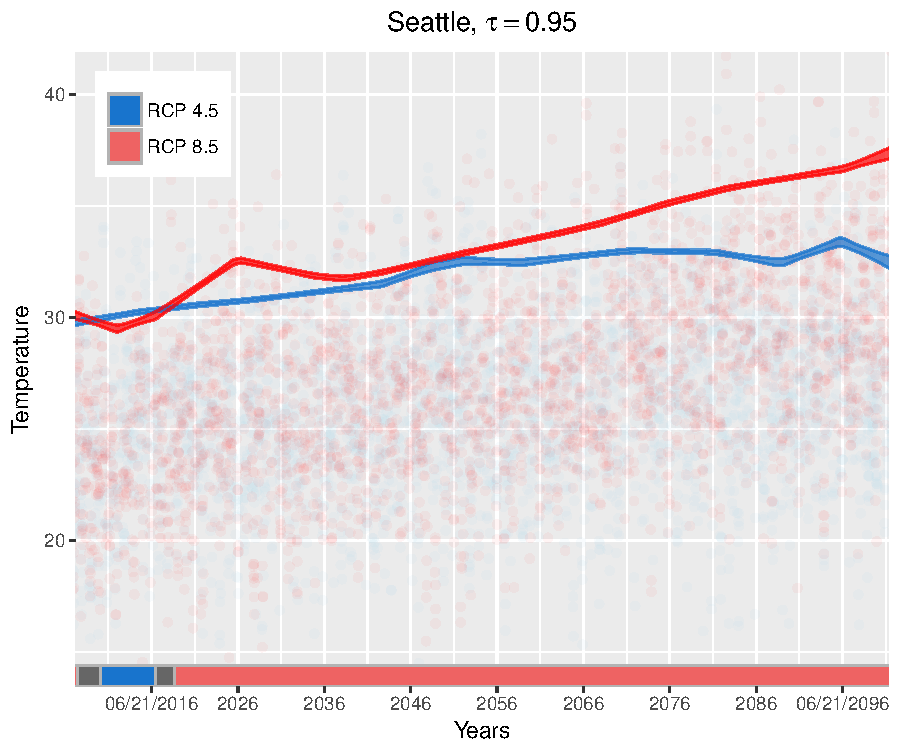
\includegraphics[width=70mm]{T0_95.pdf}}
  
  \subfigure[Difference (\SI{}{\celsius})]{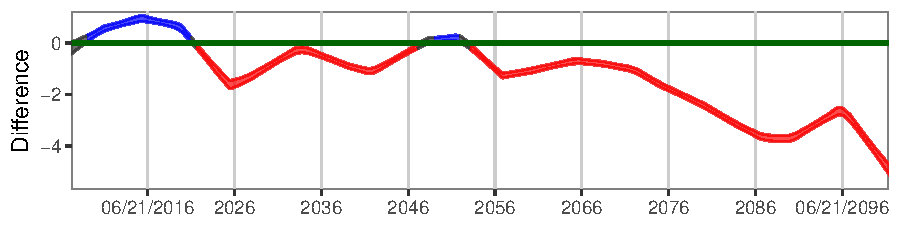
\includegraphics[width=70mm]{D0_5.pdf}}
  \subfigure[Difference (\SI{}{\celsius})]{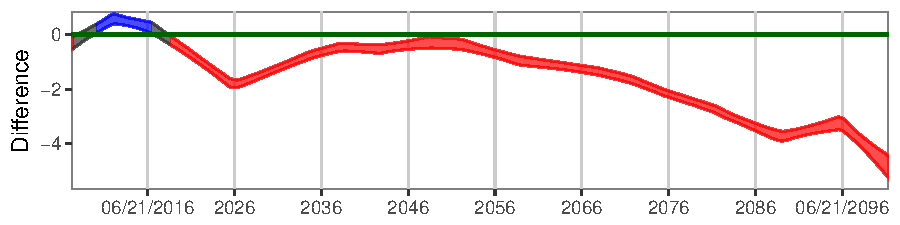
\includegraphics[width=70mm]{D0_95.pdf}}
\caption{Comparative experiment with one covariate (Seattle data). Here we include the  confidence bands computed for RCP 4.5 and RCP 8.5, and also the confidence bands  {on} the difference between the two RCP scenarios (bands appear almost as lines due to the large sample sizes). Intervals for medians ($\tau=0.5$) are on the left, and those for extreme temperatures ($\tau=0.95$) are on the right. In the stripes along the x-axes in (a) and (b), red corresponds to time periods within 2006-2100 where the RCP 8.5 scenario (the ``control")  results in higher predicted temperatures, blue corresponds to times when the RCP 4.5 scenario (the ``treatment") results in higher temperatures, and gray corresponds to periods when there is no clear `win' between the two scenarios. The bottom two plots indicate the confidence bands (RCP 4.5 $-$ RCP 8.5) on the difference.}
\label{fig:onedim}
\end{figure}
The results are presented in Figures \ref{fig:onedim} and \ref{fig:onedim_chicago}. Overall, we observe a relatively constant increase in temperature over time for RCP 8.5. For both median and extreme temperatures, there is some difference between the two scenarios in both cities, with RCP 8.5 always generating temperatures higher than those from RCP 4.5 after around 2050, which agrees with the projected developments in emissions and concentrations under these scenarios. As time increases, the difference between the two scenarios in Seattle steadily increases, whereas the difference between the two scenarios in Chicago almost drops to 0 by the end of the century.
\begin{figure}[H]
\centering   
  \subfigure[Temperature (\SI{}{\celsius})]{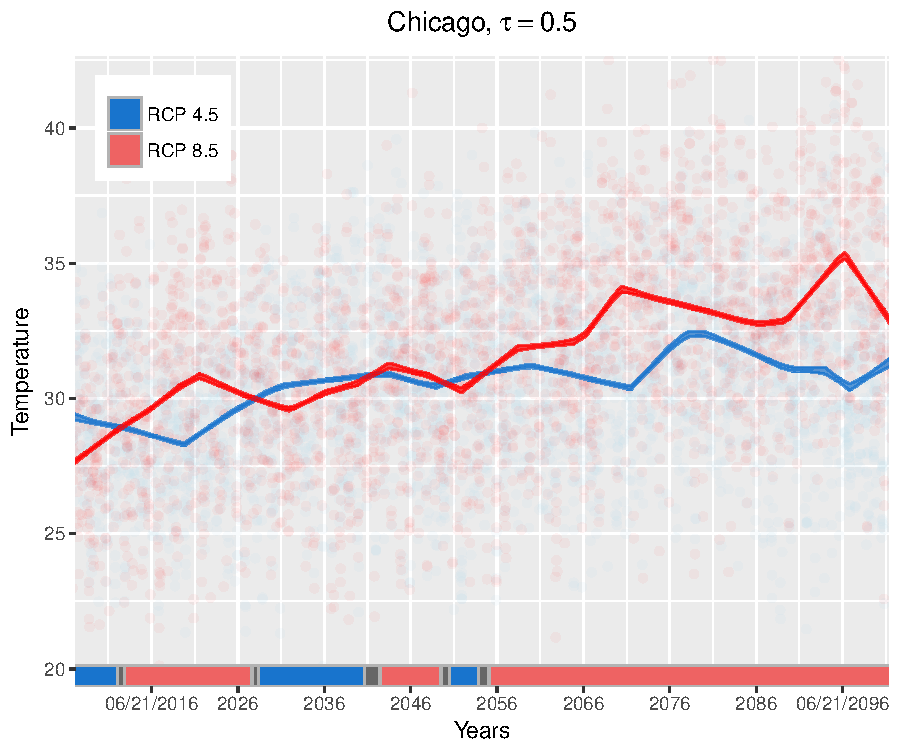
\includegraphics[width=70mm]{CT0_5.pdf}}
  \subfigure[Temperature (\SI{}{\celsius})]{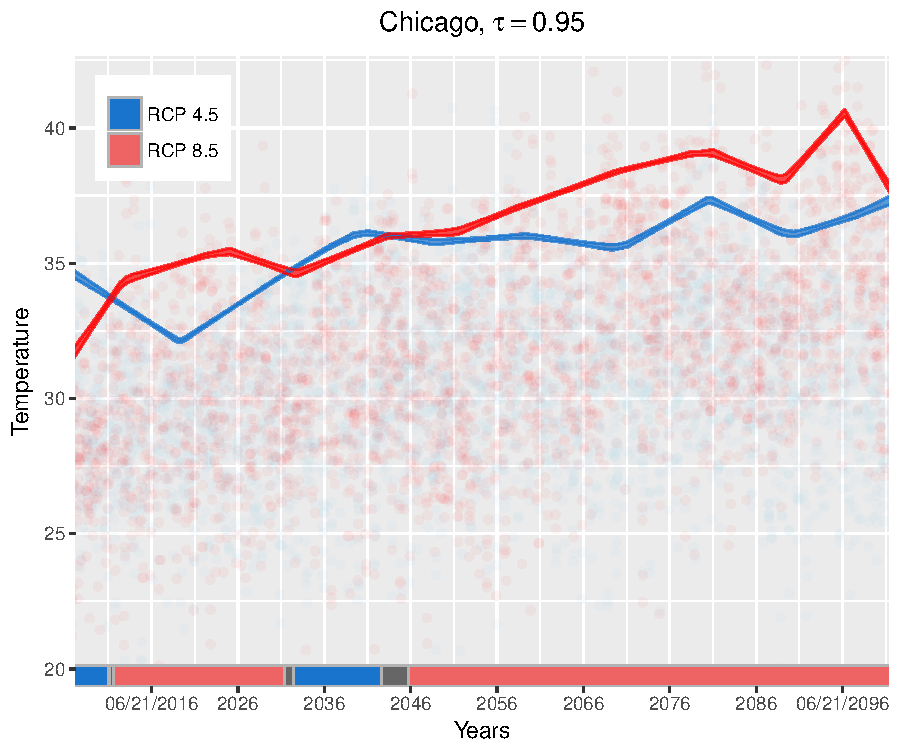
\includegraphics[width=70mm]{CT0_95.pdf}}
  
  \subfigure[Difference (\SI{}{\celsius})]{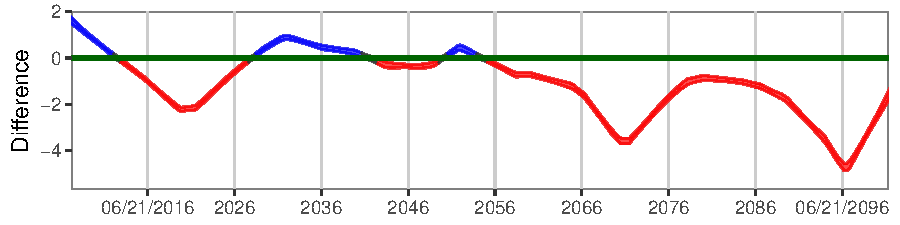
\includegraphics[width=70mm]{CD0_5.pdf}}
  \subfigure[Difference (\SI{}{\celsius})]{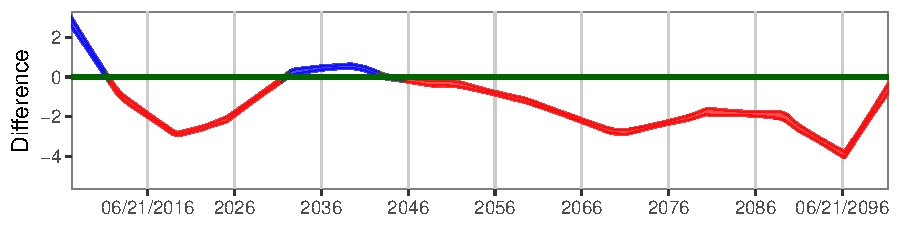
\includegraphics[width=70mm]{CD0_95.pdf}}
\caption{Comparative experiment with 1 covariate (Chicago data).}
\label{fig:onedim_chicago}
\end{figure}

\subsection{Comparative experiment with two covariates}\label{USA}

We now model the daily maximum temperature as a function of longitude and latitude at all grid points in the contiguous USA. There are 13,762 grid points in total with the spatial resolution of the NEX-GDDP data set. In the analysis, we consider all summertime daily temperature projections over the period of a decade. As a result, there are {\bf 12,661,040} observations for each RCP scenario. To apply the BLB-CVB method on the two data sets separately, we take $s=\lceil n^{0.4}\rceil, b=\lfloor n/s \rfloor\approx n^{0.6}$ such that each BLB subsample and resample contain 18,243 distinct points at most. 

We can compare the storage savings from using our BLB-CVB implementation by referring to \citet{koenker2005frisch} who indicate how the storage requirement in bytes (log-scale) for the sparse Frisch-Newton algorithm (see section \ref{weights}) increases linearly with the sample size (log-scale). For the regular bootstrap, each \texttt{rqss} implementation would require 22.9 GB for a data set with original size $n=12,661,040$. In contrast, each BLB subsample or resample requires only 0.03 GB since $b=18,243$. Consequently, the cost of computing the penalized triogram solution for each BLB resample is substantially lower.

\begin{figure}
\centering   
  \subfigure[RCP 4.5, $\tau=0.5$]{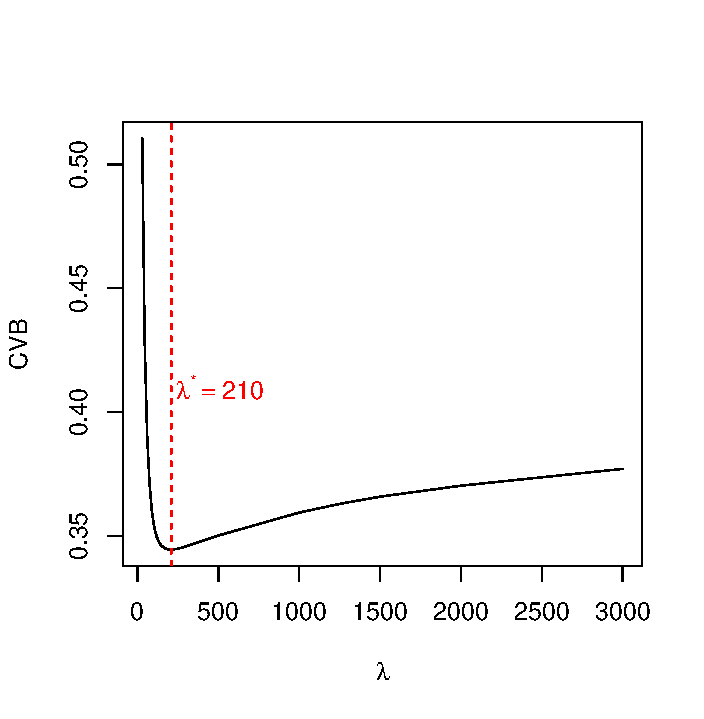
\includegraphics[width=70mm]{CVB_ct05.pdf}}
  \subfigure[RCP 4.5, $\tau=0.95$]{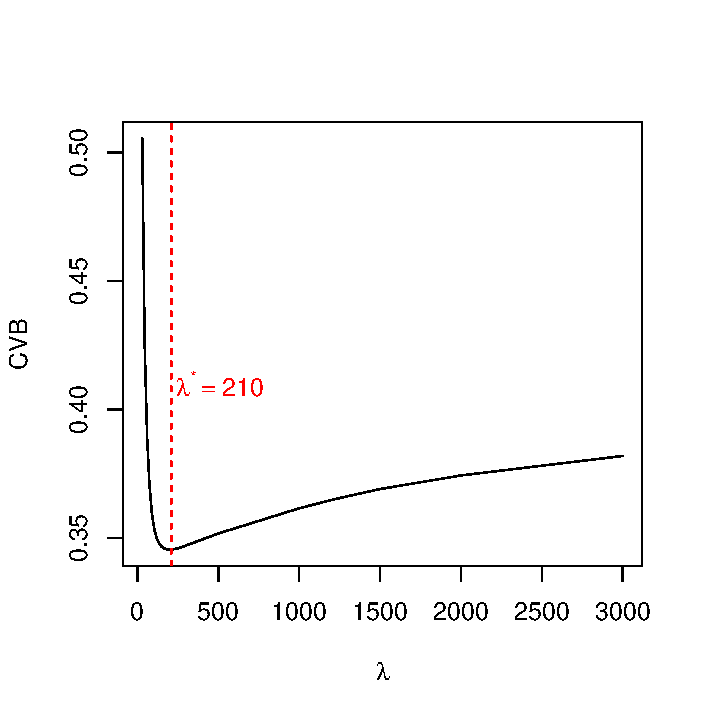
\includegraphics[width=70mm]{CVB_ct95.pdf}}
  
  \subfigure[RCP 8.5, $\tau=0.5$]{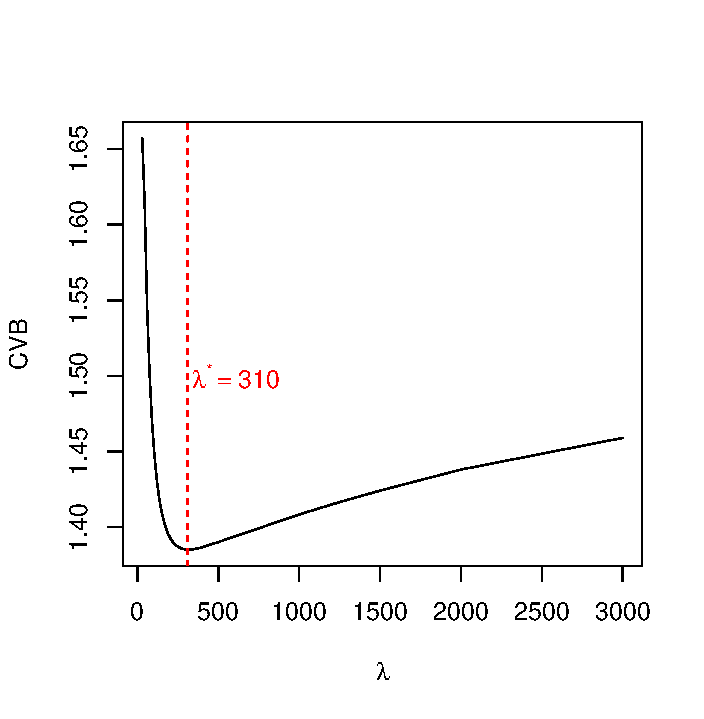
\includegraphics[width=70mm]{CVB_tr05.pdf}}
  \subfigure[RCP 8.5, $\tau=0.95$]{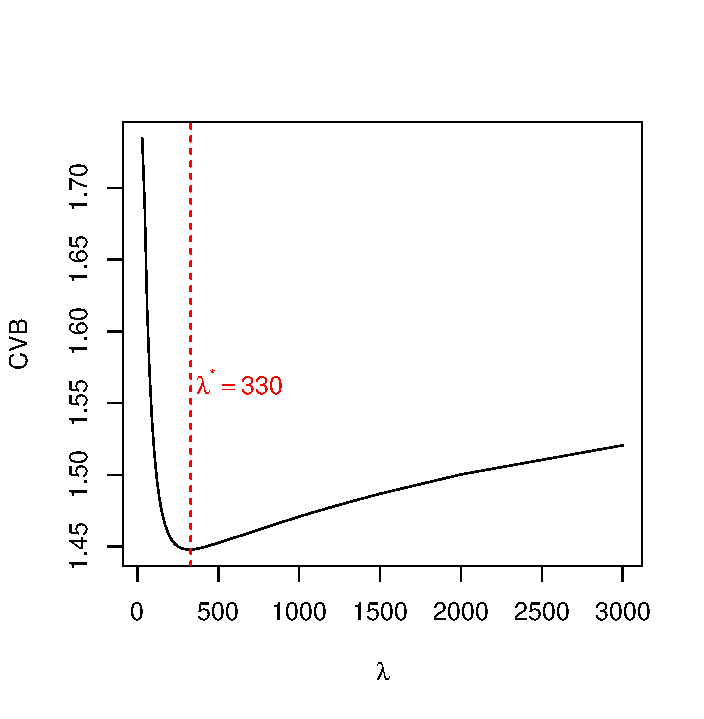
\includegraphics[width=70mm]{CVB_tr95.pdf}}
\caption{CVB calculated for two large data sets (RCP 4.5 \& RCP 8.5) each with $n=12,661,040$. The parameters for the BLB process are: $s=\lceil n^{0.4}\rceil,b=\lfloor n/s\rfloor$. We can see that  CVB$(\lambda)$ is very smooth and therefore easy to optimize.}
\label{fig:MCV}
\end{figure}
Figure \ref{fig:MCV} shows how the optimum smoothing parameters are chosen under $\tau=0.5$ and $\tau=0.95$ for each data set. These plots and other numerical experience indicate that the CVB statistic is better behaved or smoother in the case of two covariates than in the case of one covariate  {(compared with Figure \ref{fig:blb5000})}. 

Since it is difficult to present the two sets of confidence surfaces in one figure clearly, we create a difference contour plot that indicates whether RCP 8.5 or RCP 4.5 results in higher temperatures, and by how much, over the spatial domain. The results are shown in Figure \ref{fig:2dim_50} for the 2041-2050 period and Figure \ref{fig:2dim} for the 2091-2100 period. We can see that in thirty years, unremitting greenhouse gas emissions (RCP 8.5) will start to increase the temperature by 1\SI{}{\celsius} in the Pacific West and Atlantic South compared to stabilized emissions (RCP 4.5). By the end of the century, the RCP 8.5 scenario (the control) yields a higher temperature than the RCP 4.5 scenario (the treatment) over the entirety of the contiguous USA. At no location does RCP 4.5 project significantly higher temperatures for either $\tau=0.5$ and $\tau=0.95$.   {The differences between the two end-of-century projections are largest in the western basins and plateaus, with the median temperature increasing gradually from the west coasts to the Intermontane Plateaus.} More extreme temperature changes are also projected by RCP 8.5 for the Appalachians.
\begin{figure}
\centering
\caption{Temperature (\SI{}{\celsius}) quantile prediction differences during \textbf{2041$\sim$2050}. \textcolor{red}{Red}: RCP 4.5 $<$ RCP 8.5; \textcolor{blue}{Blue}: RCP 4.5 $>$ RCP 8.5.}
  \subfigure[$\tau=0.5$]{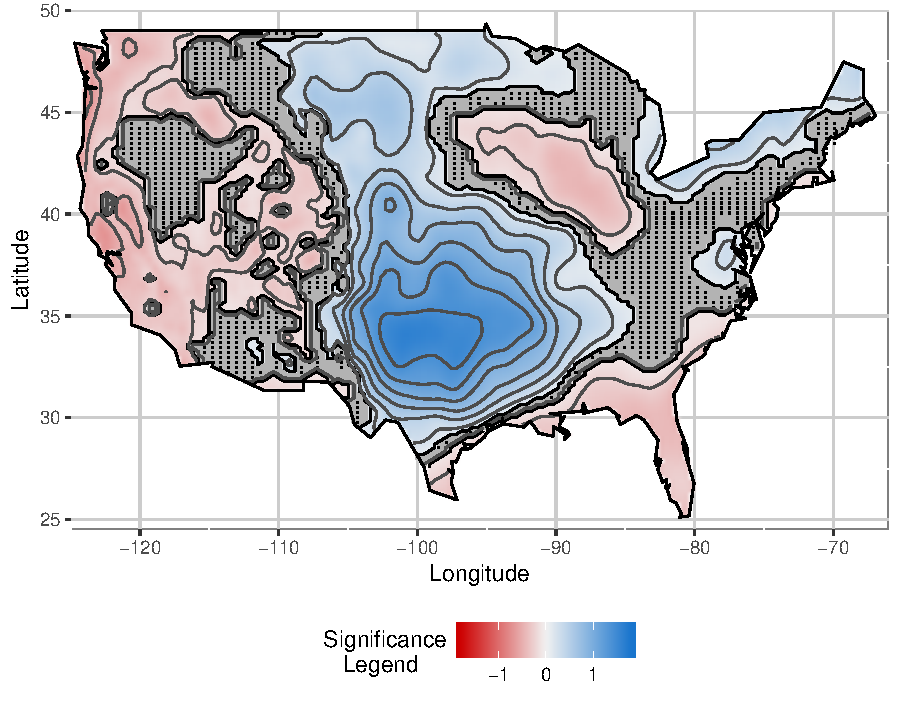
\includegraphics[width=70mm]{USA0_5_50.pdf}}
  \subfigure[$\tau=0.95$]{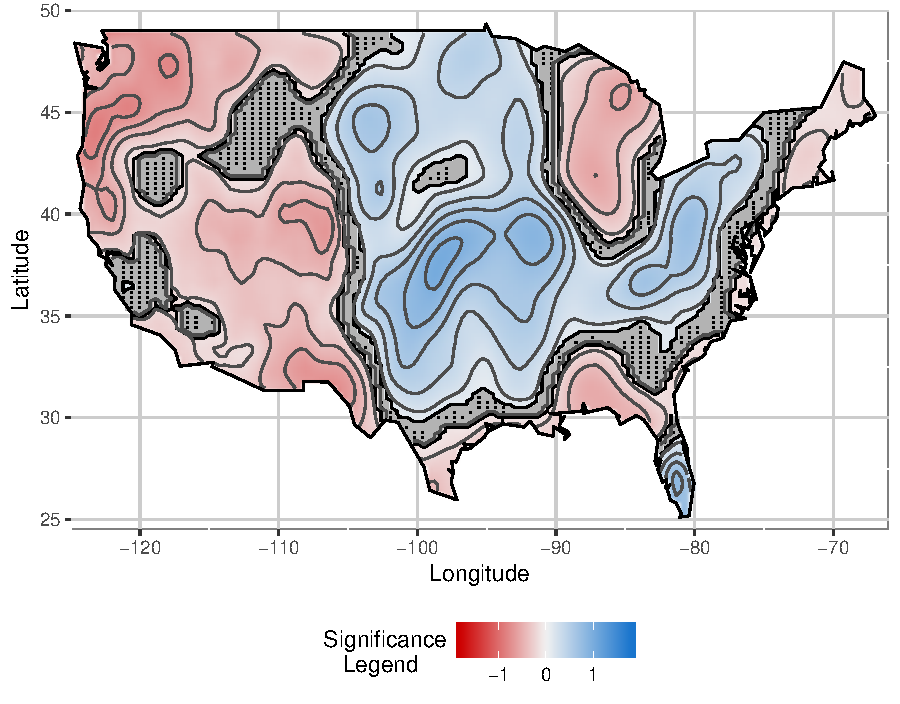
\includegraphics[width=70mm]{USA0_95_50.pdf}}
\label{fig:2dim_50}
\end{figure}

\begin{figure}
\centering
\caption{Temperature (\SI{}{\celsius}) quantile prediction differences during \textbf{2091$\sim$2100}. \textcolor{red}{Red}: RCP 4.5 $<$ RCP 8.5; \textcolor{blue}{Blue}: RCP 4.5 $>$ RCP 8.5.}
  \subfigure[$\tau=0.5$]{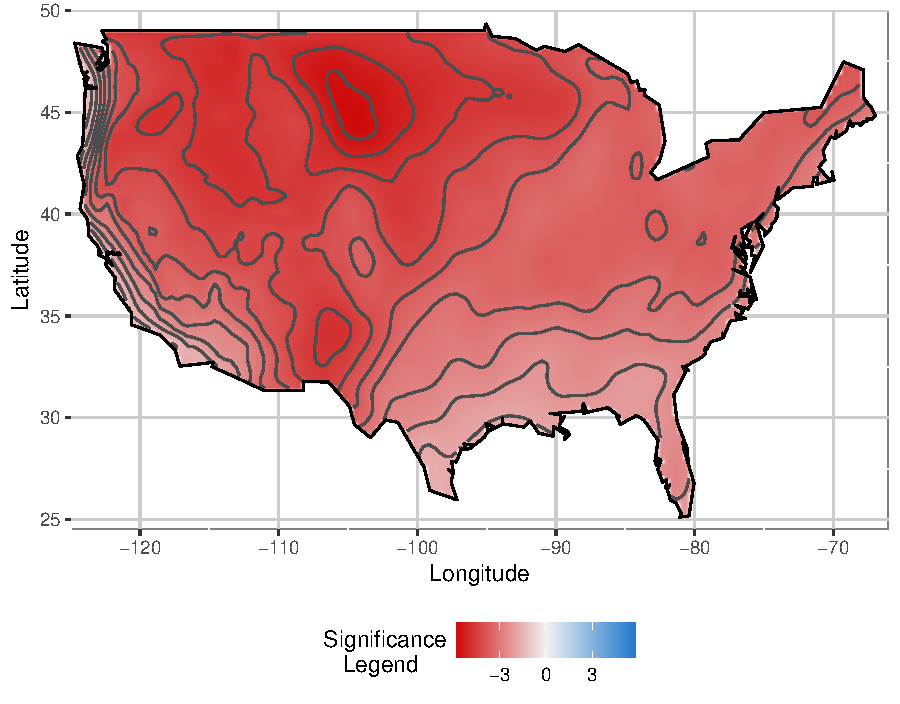
\includegraphics[width=70mm]{USA0_5.pdf}}
  \subfigure[$\tau=0.95$]{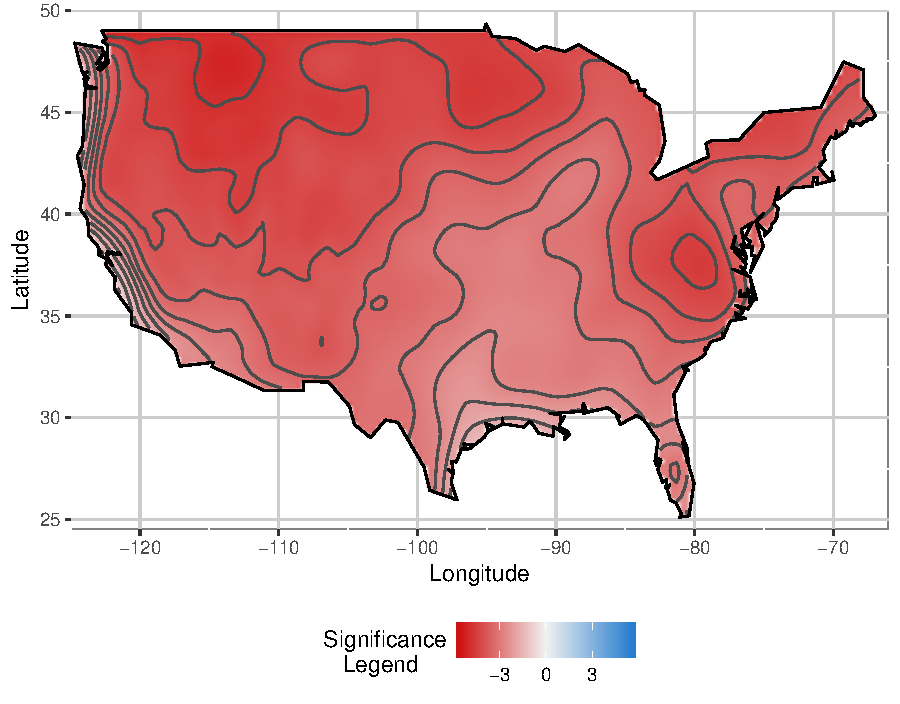
\includegraphics[width=70mm]{USA0_95.pdf}}
\label{fig:2dim}
\end{figure}

\section{Conclusion}
We have presented a new method for the computation of the confidence bands or surfaces for the quantile function estimates from massive data sets. The study has largely facilitated the study of large-scale video streaming experiments at Netflix. Our method fits penalized quantile smoothing splines to the response and computes confidence bands or surfaces via the ``bag of little bootstraps" method, specially adapted for quantile smoothing splines to take advantage of the parallel computing architecture. In particular, we presented a new cross validation criterion CVB$(\lambda)$ for determining the optimal smoothing parameter, which is easy to optimize and exploits the distributed architecture inherent in the BLB method. The resulting BLB-CVB methodology was shown to scale substantially better with the size of the data sets compared to a regular bootstrap, and to provide adequate and reliable smoothing. Coverage analyses also demonstrates the reliability of the method, and an illustration on a large climate dataset demonstrated the practical applicability of the method in the massive data setting. \textcolor{blue}{[Maybe talk about the impact on the analysis of experimentation at S\&A?]}. An R package, {\tt ConfidenceQuant} implements the methods presented in this paper.

There are various open problems for further research. We noticed  {in our numerical tests} that the CVB($\lambda$) function under two covariates appeared  smoother  (i.e., it is better behaved) than when only one covariate is used, and this requires further investigation. Extending the present method to more than two covariates is a  {challenging} matter for further research. 

\subsection*{Acknowledgements}
Climate scenarios used were from the NEX-GDDP dataset, prepared by the Climate Analytics Group and NASA Ames Research Center using the NASA Earth Exchange, and distributed by the NASA Center for Climate Simulation (NCCS).

\bigskip
\begin{center}
{\large\bf SUPPLEMENTARY MATERIAL}
\end{center}

\begin{description}

\item[Title:] ConfidenceQuant.tar.gz

\item[R-package for the BLB-CVB routine:] R-package ConfidenceQuant containing code to select optimum smoothing parameter when fitting penalized quantile smoothing splines, compute confidence bands or surfaces for large data sets, and visualize the results with the help of \texttt{ggplot} and \texttt{plotly}. The package also contains the simulated set shown in figure \ref{fig:edf} used as examples throughout the article (\texttt{demo.csv}). Besides, a user guide file with detailed explanations on each function and a package vignette file that goes through every function very quickly are included in the package to help users try out the functions. Users can also invoke the help pages of the functions to learn about the input parameters and run through the sample code.

\end{description}
\bibliographystyle{rss}
\bibliography{main}
\end{document}